\chapter{\label{I_2}Implémenter le FRBR adapté aux archives audiovisuelles au sein d’un outil de gestion des collections} 

%I 2 

%Reprendre la définition du logiciel de gestion des collections ? Pour montrer que le FRBR aide à la gestion des collections 

Comme défini en introduction, un logiciel de gestion des collections est un outil “spécialisé permettant de gérer des informations structurées” \footcite{zotero-item-766}. De ce fait, il structure le système d’information qui permet à une institution d’orchestrer le cycle de vie de sa collection. Cette structuration des données doit être modélisée selon les spécificités propres au type de collection d’un institution cliente, à partir de normes descriptives définies et de cadres de référence pour l’indexation des collections. Dans le cas des archives audiovisuelles, le logiciel des gestions des collections devrait ainsi permettre une structuration de l’information adaptée au type de corpus conservé, respectant toutefois le cadre de référence pour la modélisation des données, le FRBR. La restructuration du modèle de données permet de construire pour l’utilisateur, un logiciel de gestion des collections intelligible avec des outils de recherche performants. (En accord avec les besoins utilisateurs FRBR)  


\section{\label{I_2_A}Un espace de travail dédié à la gestion de collections audiovisuelles : S-Movies}

Si le manuel de la FIAF pose le cadre d’une adaptation du modèle FRBR pour la gestion des archives audiovisuelles, il s'agit désormais de confronter ce cadre à une implémentation concrète. Pour cela, nous analyserons au cours de ce chapitre l’implémentation d’une telle modélisation au sein d’un outil de gestion des collections, celui développé par Skinsoft. Nous y analyserons spécifiquement l’espace de travail développé pour la gestion des archives audiovisuelles : S-Movies. En effet, le contexte de notre étude se situe principalement dans le cadre de l’analyse de cet espace de travail afin d’en analyser la modélisation, en vue de l’améliorer et d’y implémenter potentiellement des fonctionnalités automatiques, fondées sur l’intelligence artificielle.  

Présentons d’abord le fonctionnement général de l’outil de gestion des collections développée par Skinsoft. Celui-ci est divisé en espaces de travail, chacun dédiés à un type de collection, comme le montre la capture d'écran de la page d'accueil ci-dessous (\ref{figAccueil}). (dire en note de bas de page que les captures viennent d’une appli de test configurée par nos soins)

\begin{figure}[htbp] 
	
	\centering 
	
	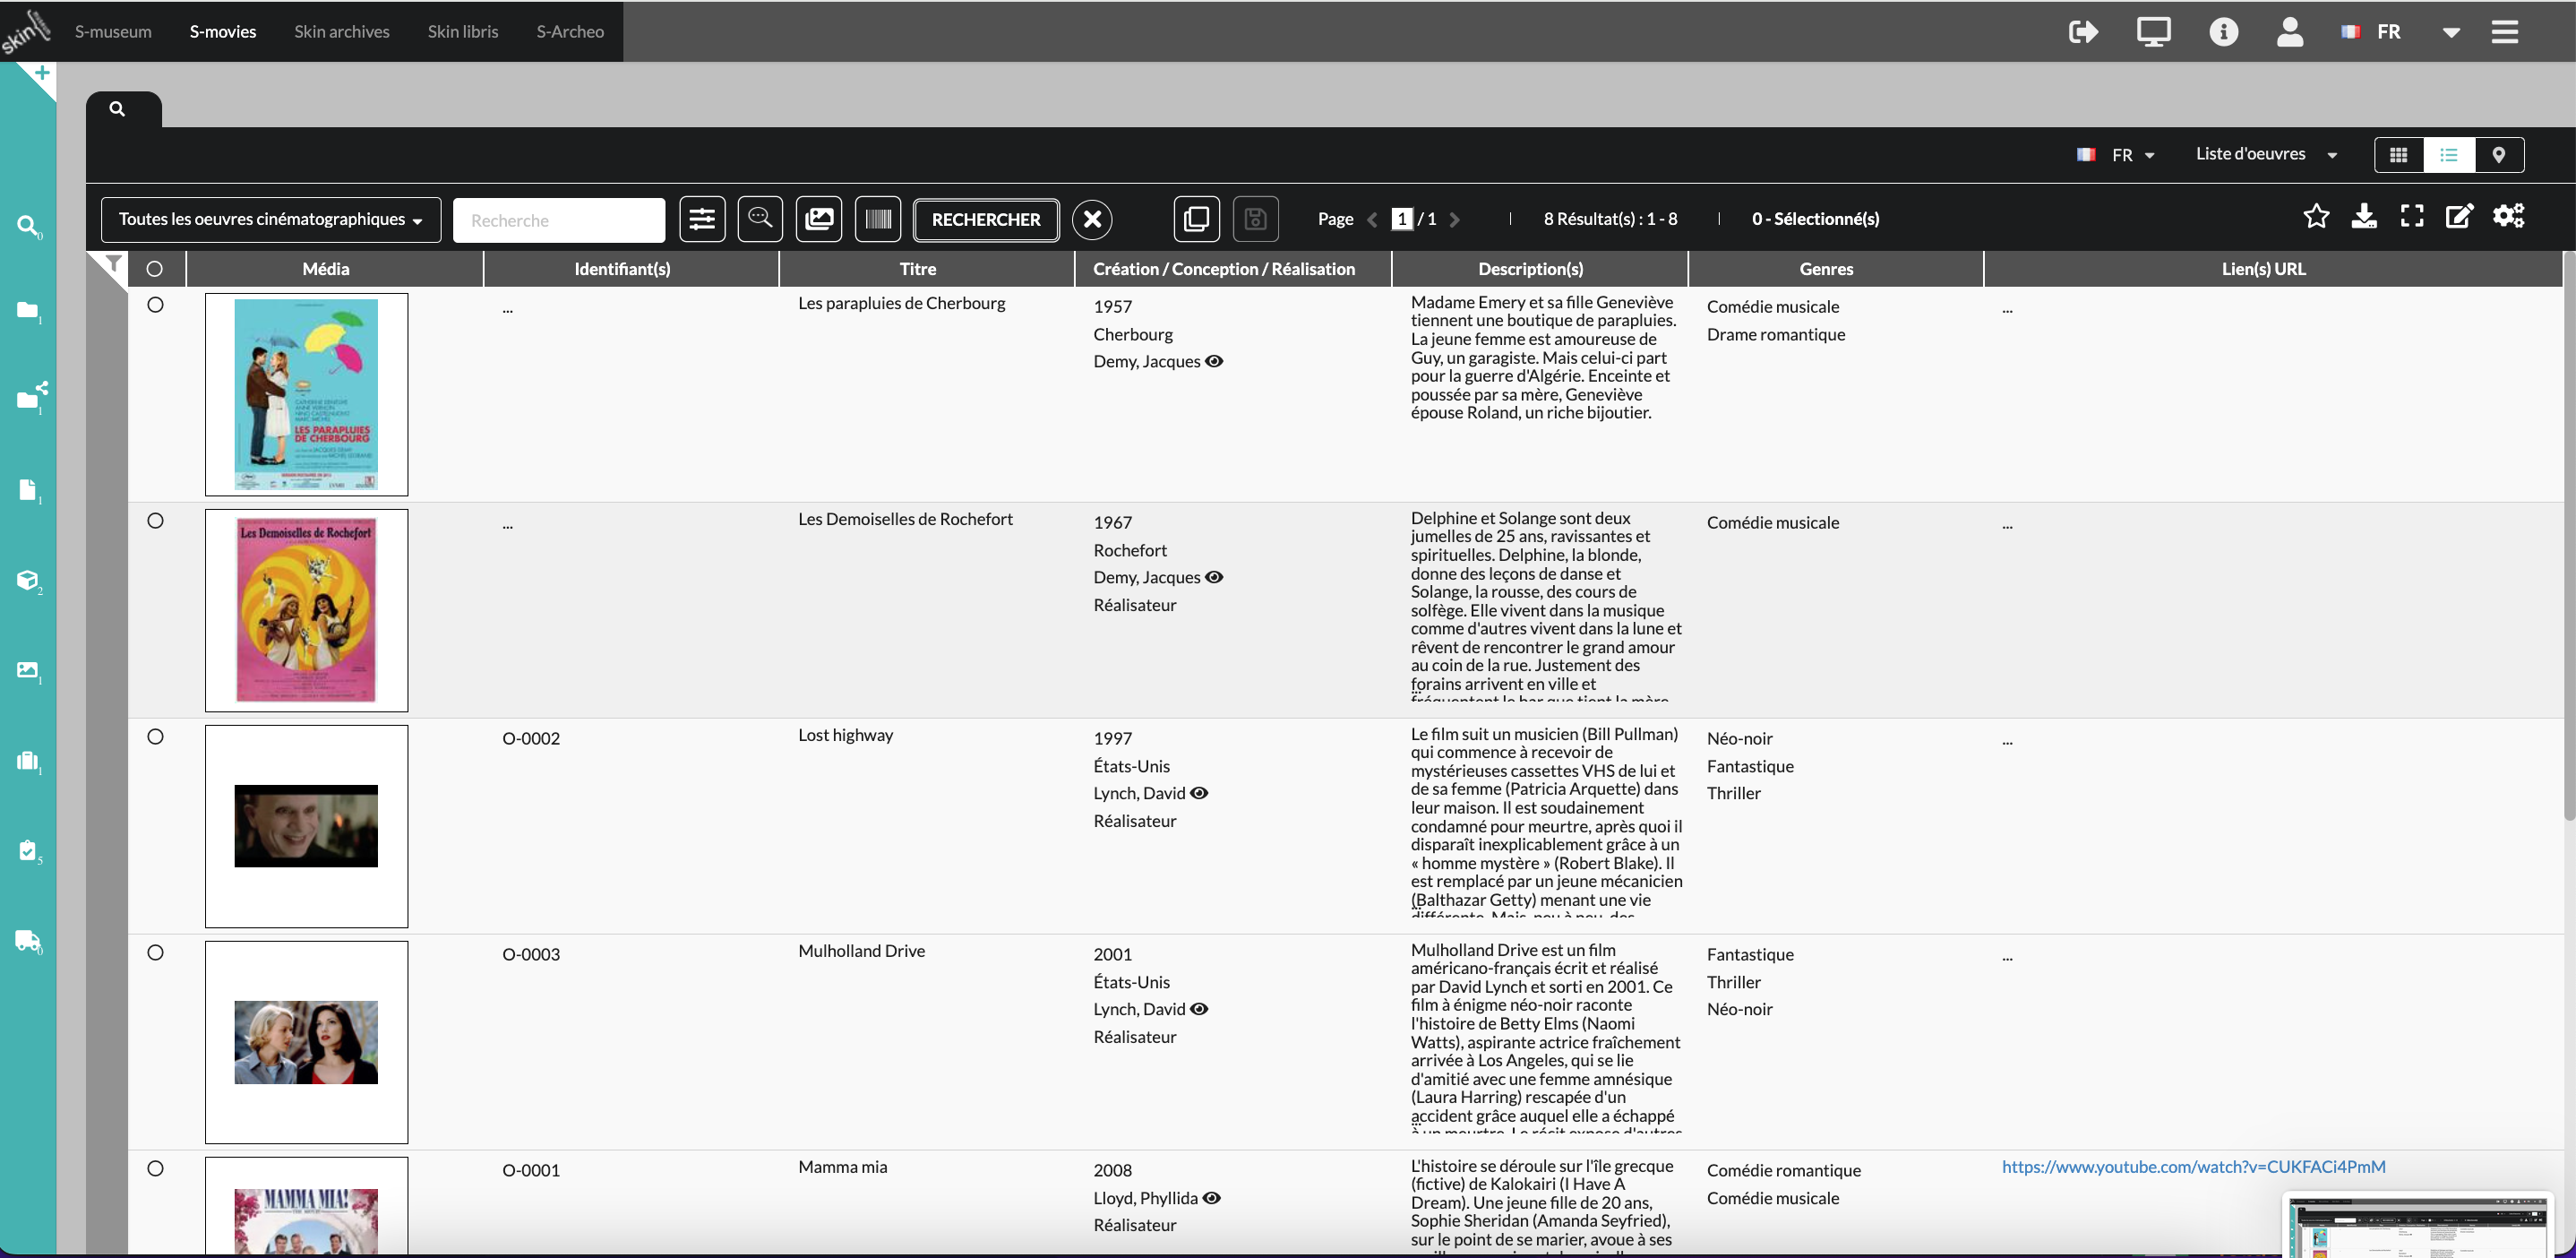
\includegraphics[width=0.85\textwidth]{images/image.png} 
	
	\caption{Page d'accueil de l'espace de travail} 
	
	\label{figAccueil} 
	
\end{figure}

Une institution cliente de l’outil peut combiner un ou plusieurs espaces de travail, selon les données à gérer. Cette structure permet justement d’adapter l’interface à chaque type de collection géré : objets de collection de musée, collections archéologiques, collections de films, collections bibliographiques, collections d’archives, etc. Chaque espace de travail permet notamment la gestion des acquisitions, des collections, de leurs mouvements, de projets, d’expositions, des médias... De plus, chaque espace de travail est structuré selon des normes de description et un cadre de modélisation adaptés au type de collection qui y est géré. L'espace de travail S-Movies est modélisé selon les préconisations de la FIAF sur l’adaptation du FRBR, et structuré selon les normes de descriptions évoquées. Ainsi, les collections sont organisées en trois entités distinctes, conformément aux adaptations du FRBR par la FIAF : Films, Manifestations, Œuvres cinématographiques (Films désigne ici le niveau Item), comme le montre la capture d'écran du menu de l'espace de travail, ci-dessous :   

\begin{figure}[htbp] 
	
	\centering 
	
	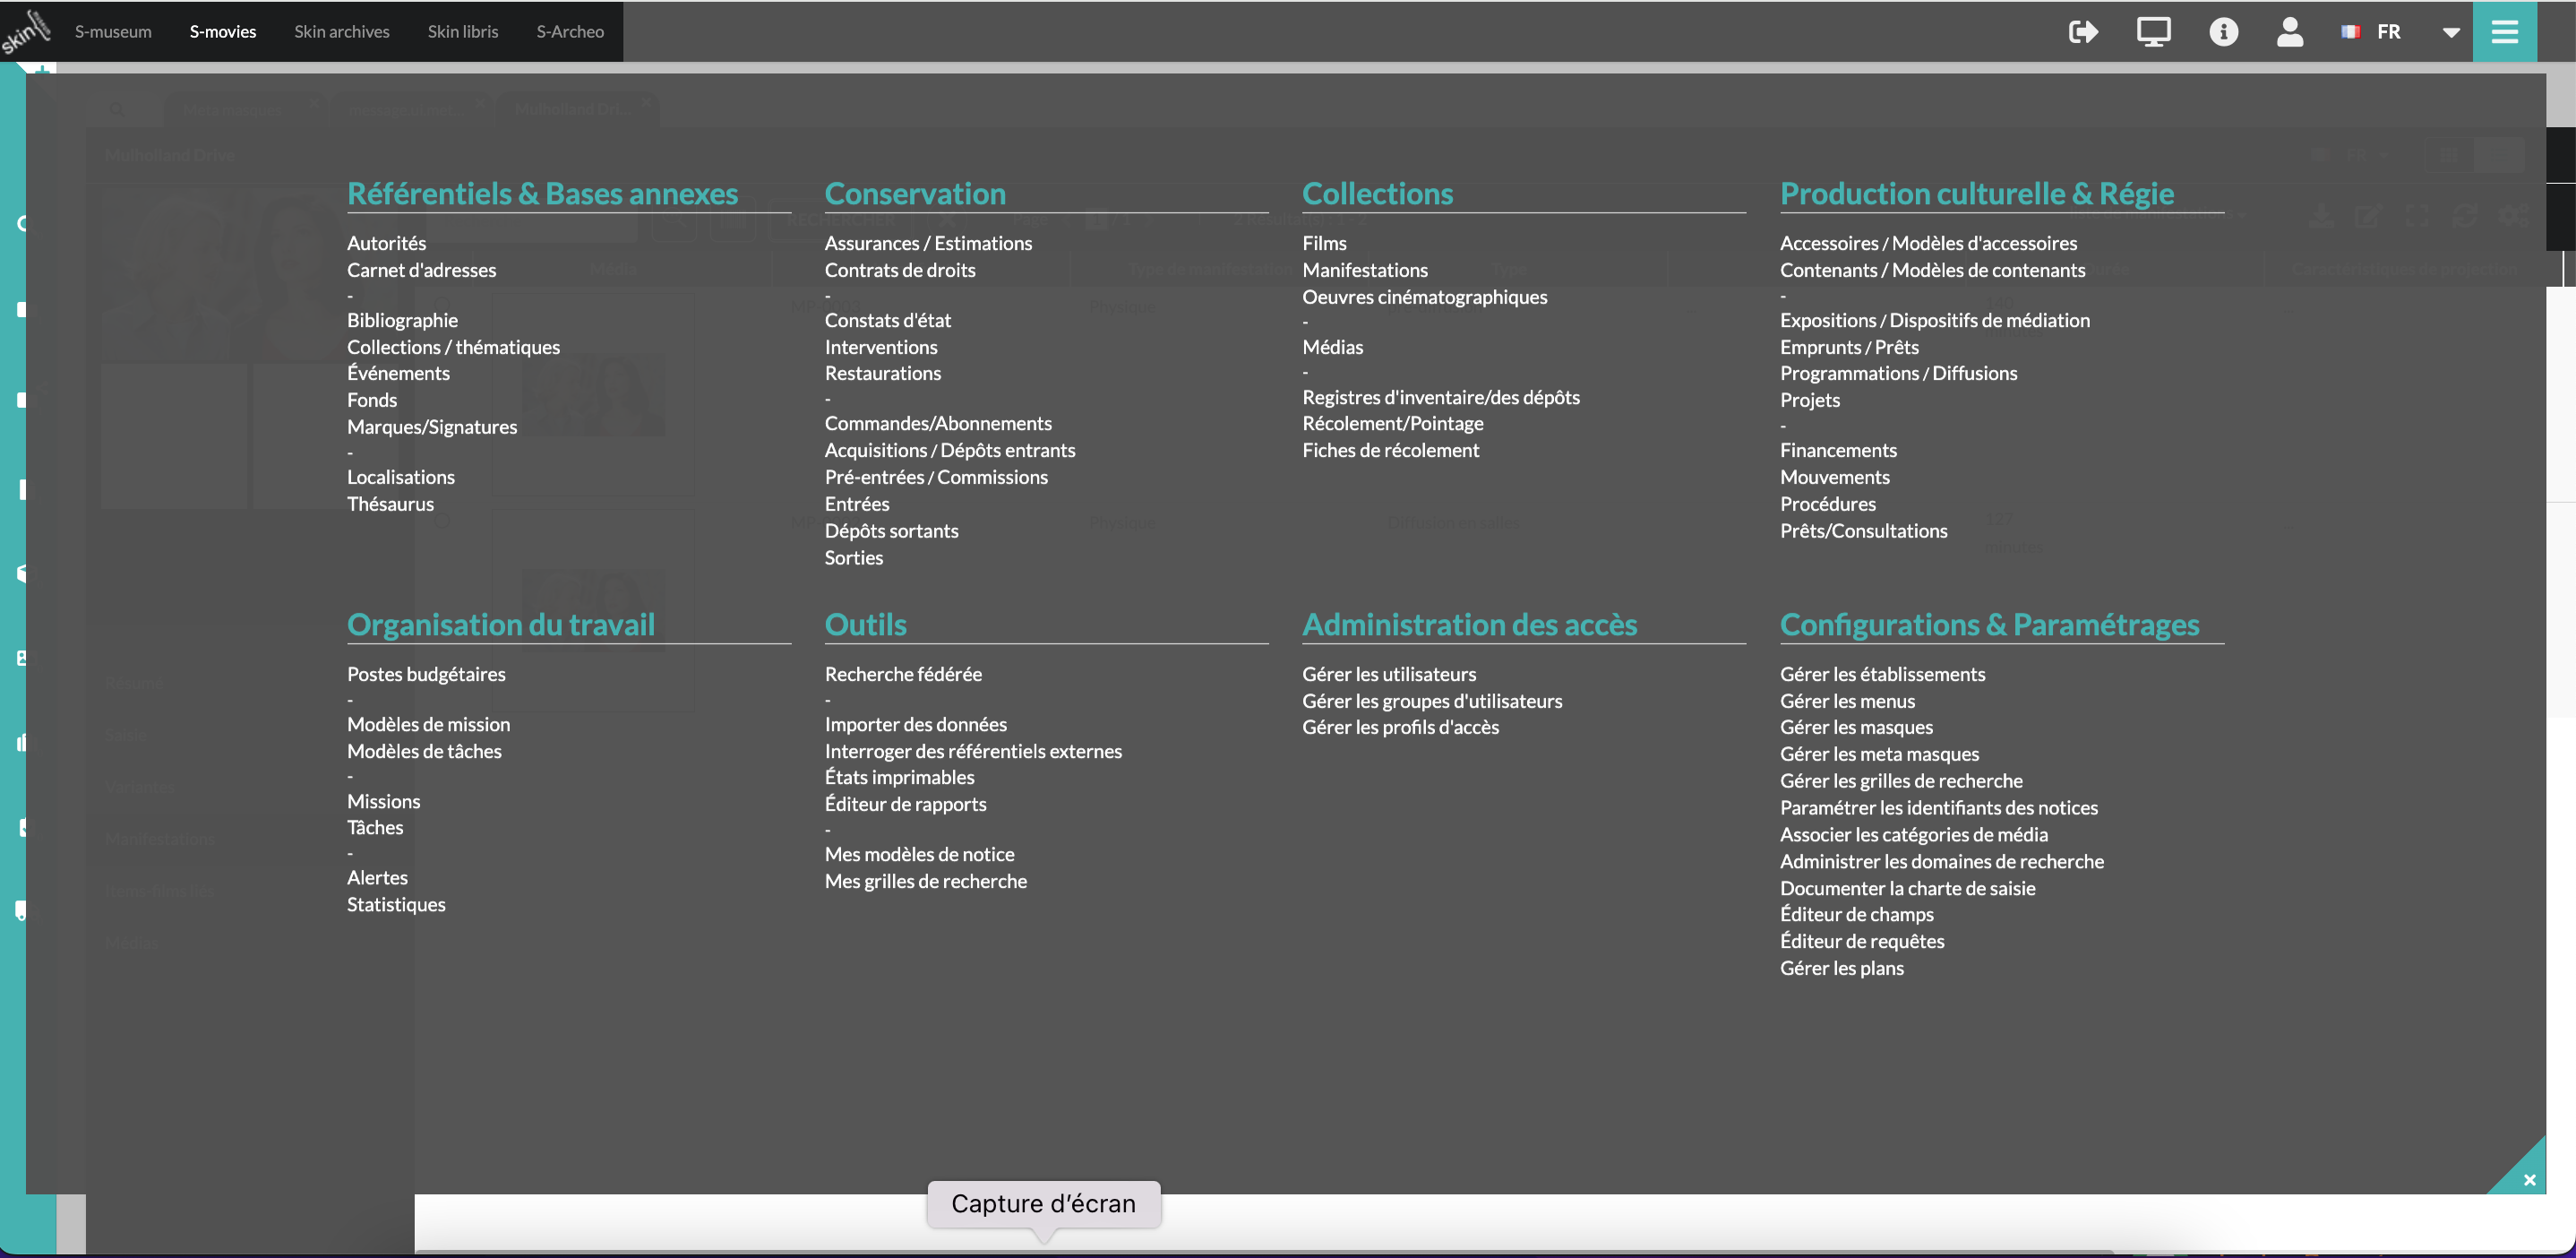
\includegraphics[width=0.85\textwidth]{images/image6.png} 
	
	\caption{Menu burger de l'espace de travail} 
	
	\label{figMenu} 
	
\end{figure}

Dans chacune de ces tables de données, l'utilisateur peut créer de nouvelles notices, et y associer des notices des autres tables. Par exemple, depuis la table Œuvres cinématographiques, l'utilisateur peut créer une notice d’Œuvre et y associer des notices de Manifestations et d'Items qui y sont directement liées. La Variante telle que définie dans le manuel de la FIAF n’est pas représentée par une entité à part entière sous la forme d’une table comme c’est le cas pour les autres entités. Toutefois, il est possible de créer une notice de Variante au sein de la table Œuvres cinématographiques, directement liée à une Œuvre. La Variante aura le même statut qu’une Oeuvre, mais elle sera de type Variante.  

Par exemple ci-dessous, une notice d’Œuvre cinématographique à laquelle sont associées deux notices de Manifestation :  

\begin{figure}[htbp] 
	
	\centering 
	
	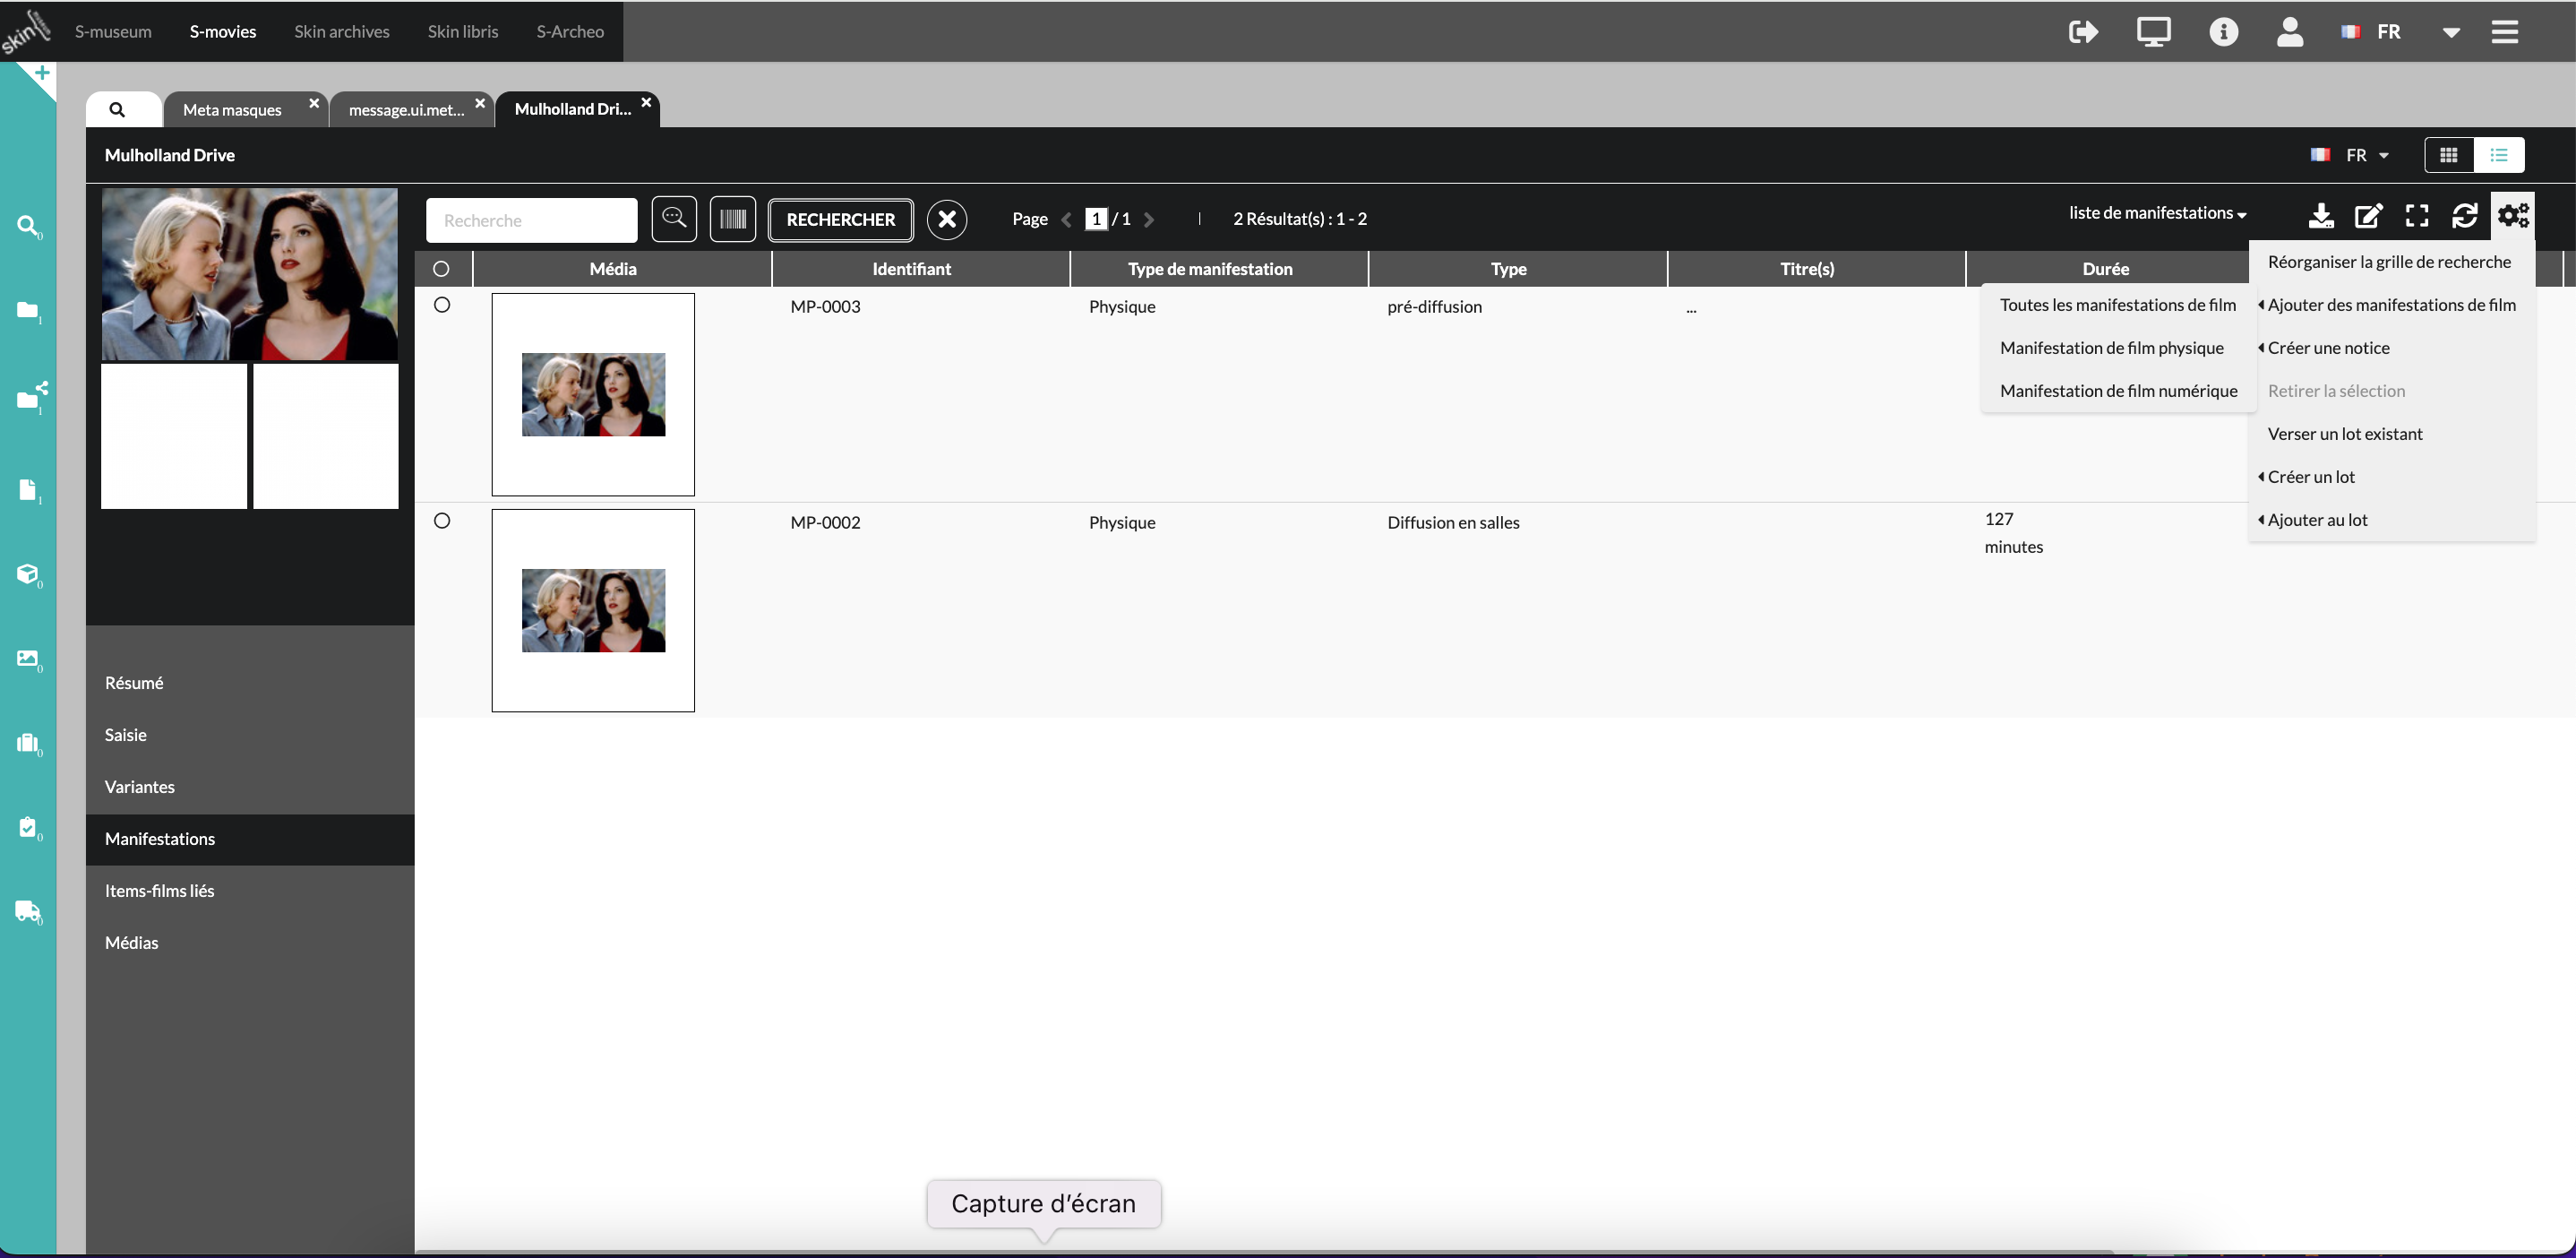
\includegraphics[width=1.0\textwidth]{images/image7.png} 
	
	\caption{Menu burger de l'espace de travail} 
	
	\label{figNoticeOeuvre} 
	
\end{figure}

L’interface permet d’associer des notices depuis un bouton d’action situé à droite.  

De plus, en fonction de la nature du corpus géré, un paramétrage adaptatif est prévu afin d’ajuster l’interface aux pratiques métier de chaque institution. En effet, une adaptation supplémentaire de la modélisation de données via la configuration flexible de chacun des espaces de travail. Trois configurations sont principalement possibles : le paramétrage de champs de saisie pour chaque type de notice, l'organisation de ces champs dans des grilles de résultats de recherche, et l'assemblage des champs et des grilles de recherche dans des menus navigables pour chaque type de notice. (Schémas explicatifs ?) Ce paramétrage concrétise la modélisation de données selon le cadre de référence utilisé.  

%quel rôle joue la modélisation dans ce cas ? En amont du paramétrage ? Ou en aval ? (Reprendre la définition) ou tout ce paramétrage fait partie de la modélisation  

Ainsi, une double adaptabilité est proposée : d’une part un espace dédié à un type de collection et structuré en fonction des normes de description et de la modélisation de données préférée, et d’autre part un paramétrage précis de l’espace de travail, propre au type de corpus géré par l'institution cliente, concrétisant ainsi la modélisation de données propre qui sera utilisée.  

L’espace de travail S-Movies est pré structuré suivant la modélisation FRBR préconisée par la FIAF. Cette structure stable, permet à Skinsoft de proposer un espace de travail pré défini pour chaque institution préservatrice de ce type de collection. En revanche, les corpus audiovisuels préservés par différentes institutions peuvent être de toutes sortes, sur différentes thématiques, sous différents formats. Cette hétérogénéité suppose des règles métiers spécifiques, issues des besoins de gestion de la collection préservé. Ainsi, par exemple, une collection audiovisuelle expérimentale ou amateure ne nécessitera pas les mêmes champs de saisie, les mêmes thésaurus, ou de la même disposition des résultats de recherche, qu'une collection audiovisuelle industrielle, grand public.   

Concrètement, au sein de l’espace de travail, la description d’un élément s’effectue au sein de champs de saisie, sélectionnés de manière adaptée aux besoins de description de l’institution donnée. Ces champs, s'ils sont paramétrables individuellement, font en réalité partie d'une structure plus large, à l'échelle de l'espace de travail dans lequel ils se situent. En effet, ces champs sont regroupés dans des masques, qui correspondent à des formulaires de saisie spécifiques au type de notice concerné. Par exemple, une notice de film physique, décrivant le niveau Item pourra contenir un masque de saisie, contenant des champs de saisie correspondants (cf \ref{figMasques}): identifiants, format de l’item, support de l’item, etc. 

\begin{figure}[htbp] 
	
	\centering 
	
	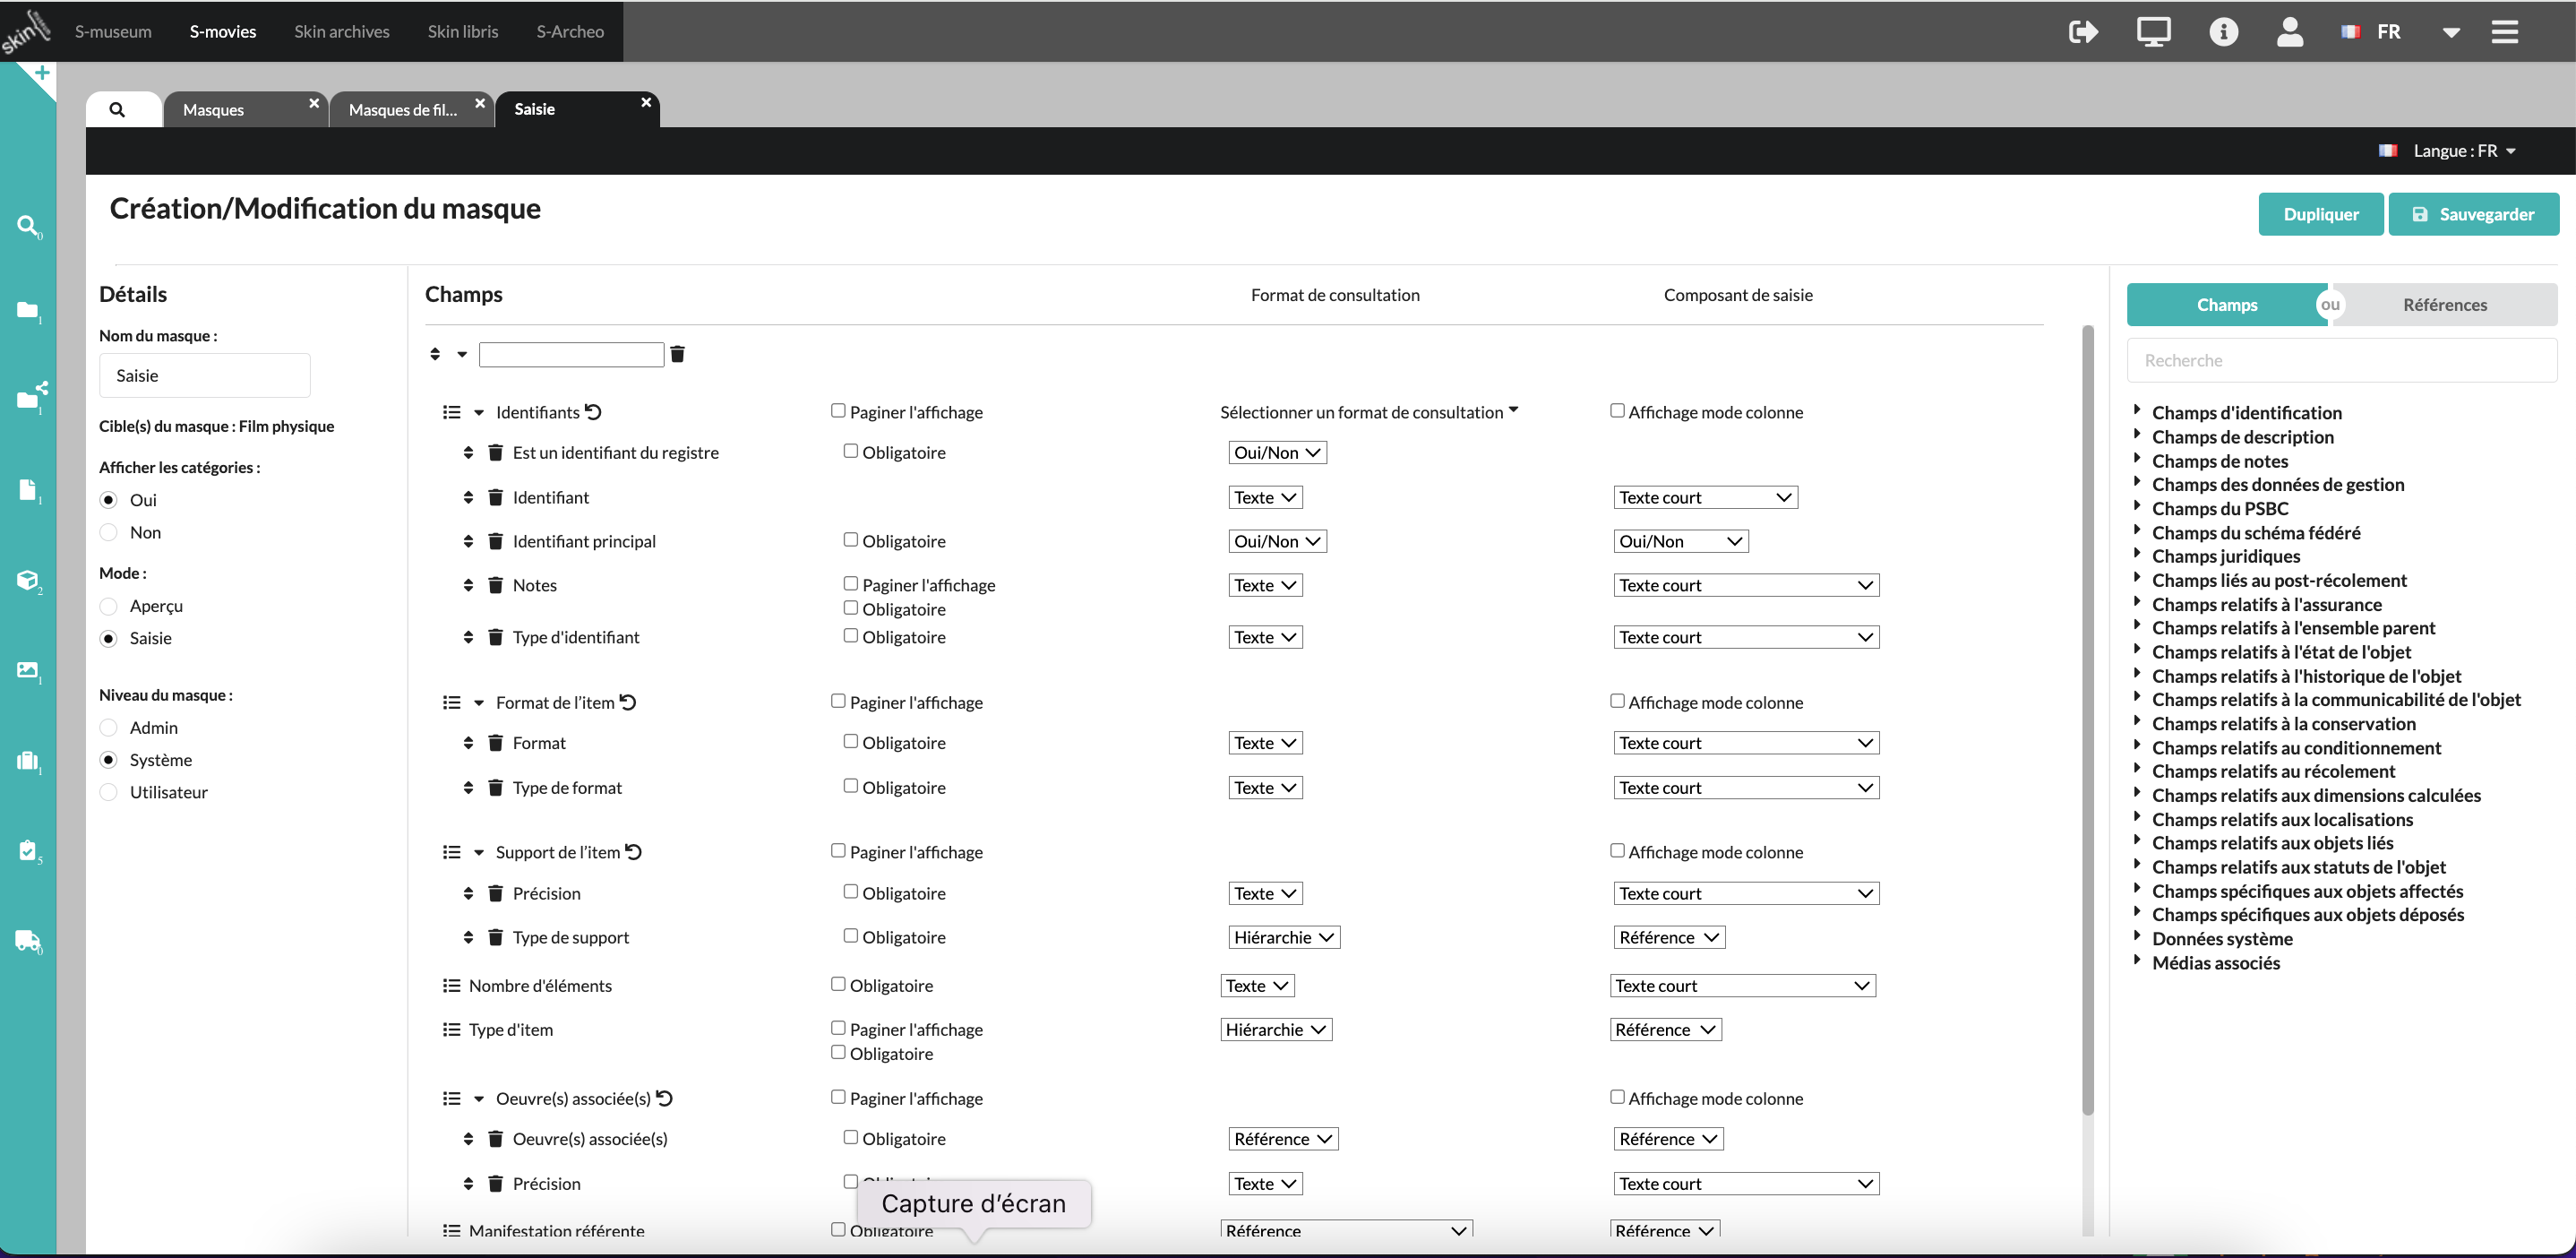
\includegraphics[width=1.0\textwidth]{images/image2.png} 
	
	\caption{Configuration des masques de saisie au niveau Item} 
	
	\label{figMasques} 
	
\end{figure}

Ce masque pourra ensuite être assemblé en tant qu’onglet au sein d’un menu d'une notice de film physique, permettant à l'utilisateur d'y remplir les champs que nous avons mentionnés. Ici, le menu d’une notice de film physique qui contient le masque de saisie mentionné plus haut :  

\begin{figure}[htbp] 
	
	\centering 
	
	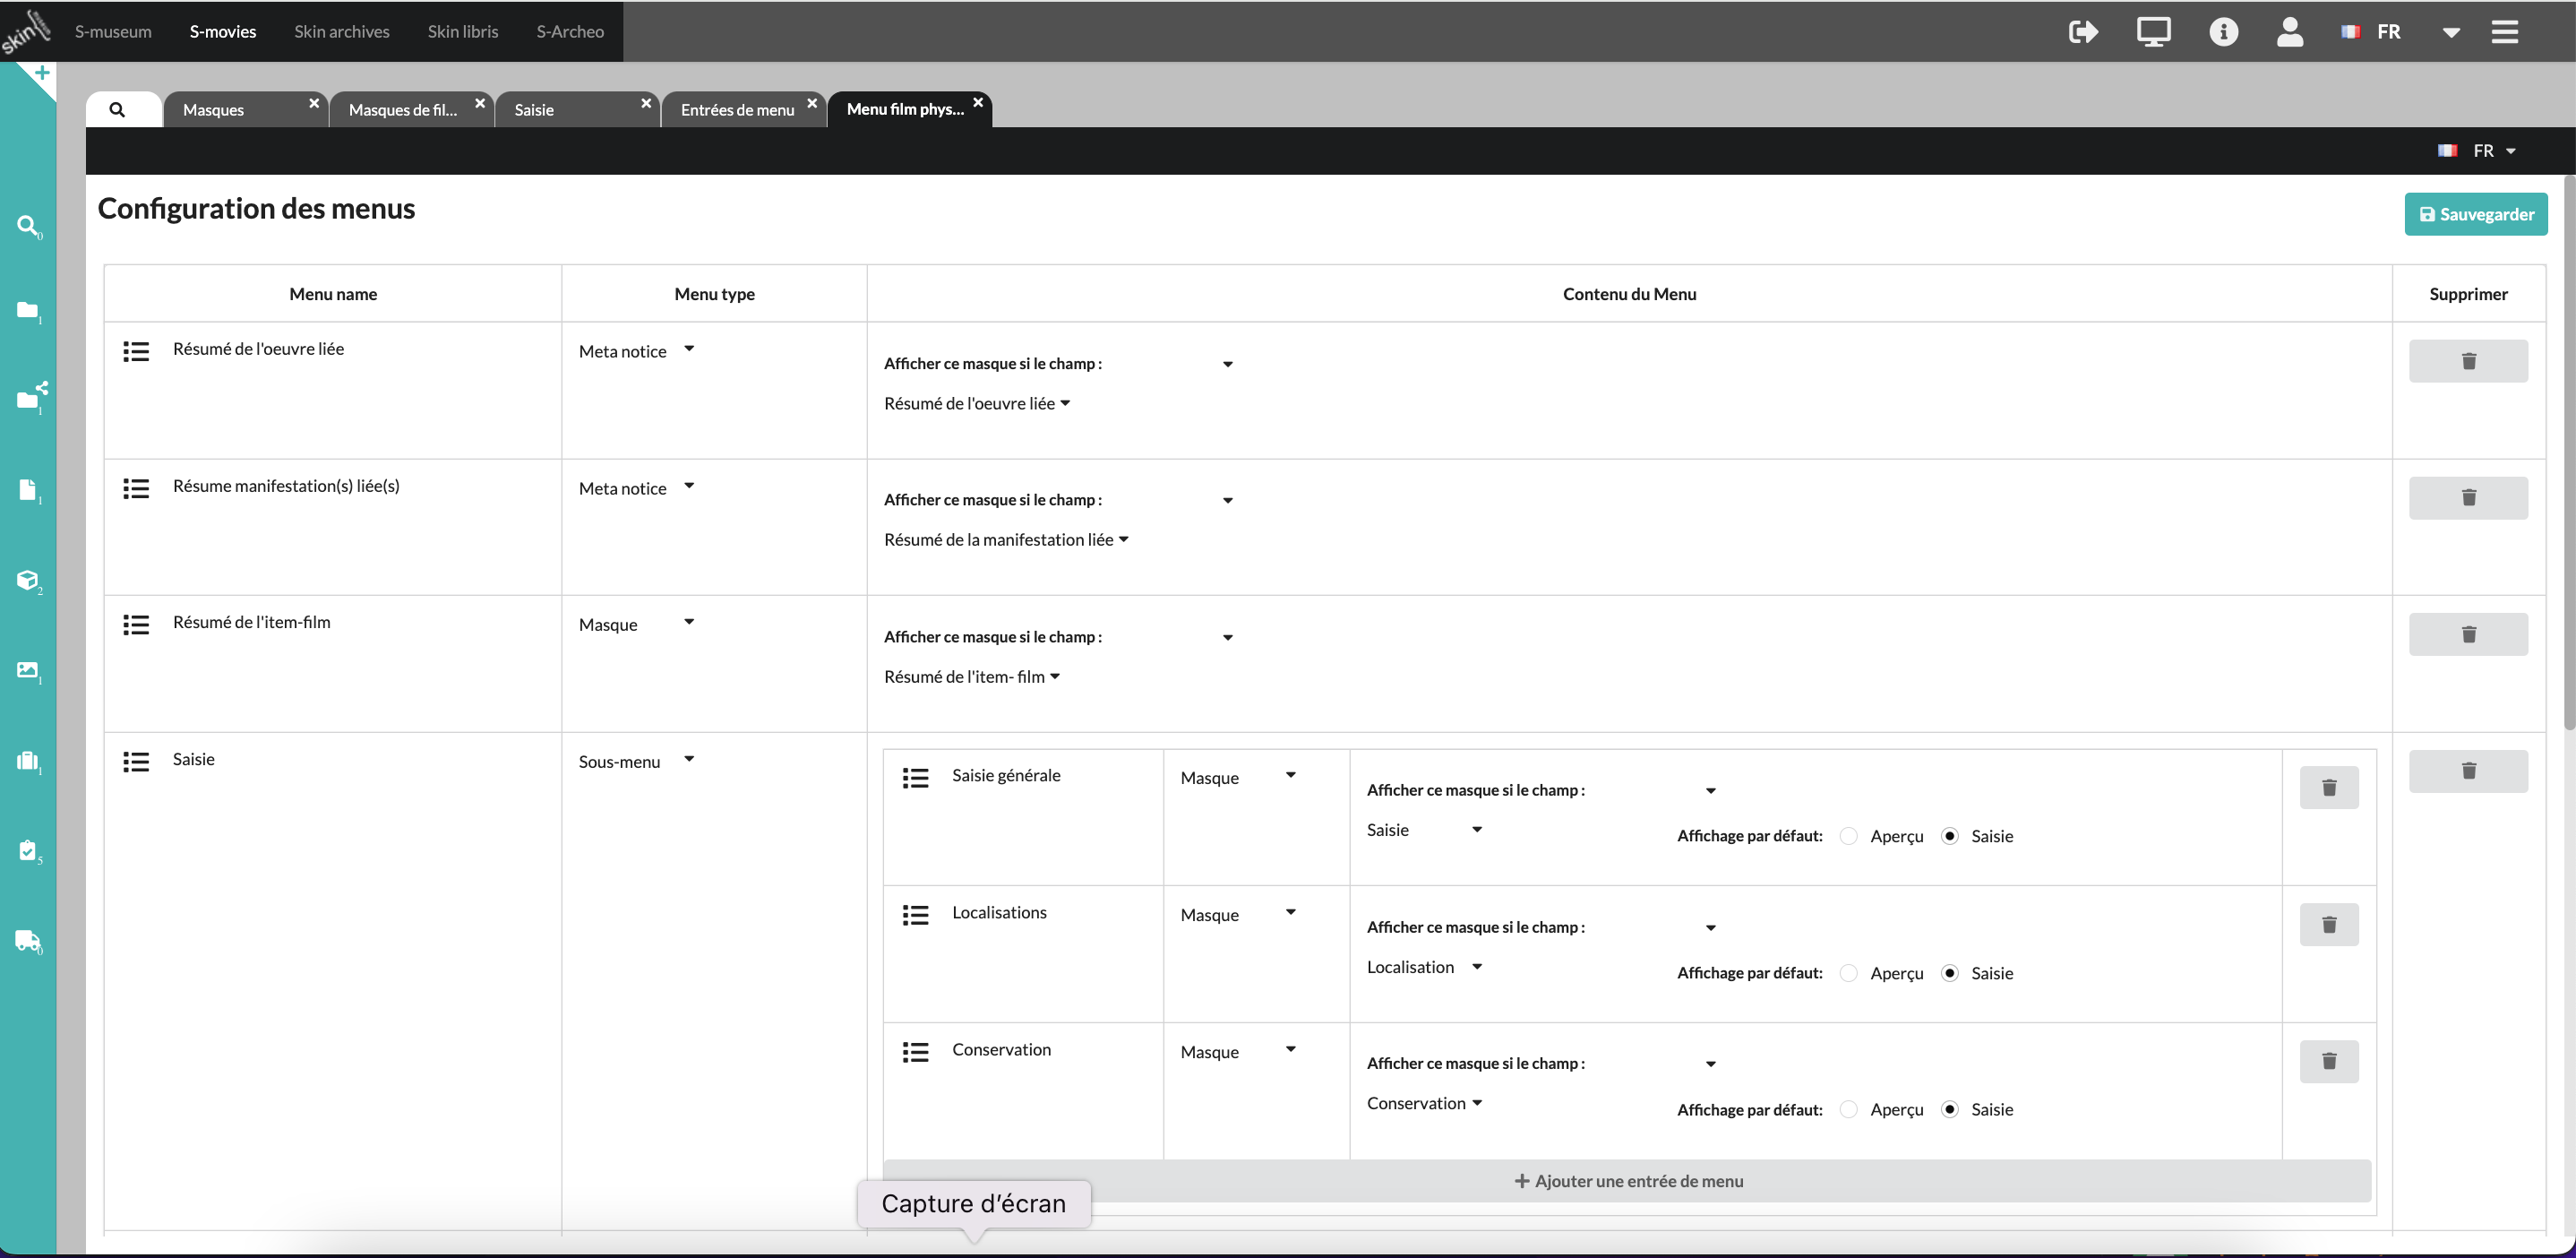
\includegraphics[width=1.0\textwidth]{images/image3.png} 
	
	\caption{Configuration du menu d'une notice de film physique} 
	
	\label{figMenuFilm} 
	
\end{figure}

Et ici la manière dont il s’affiche pour l’utilisateur, à la saisie dans une nouvelle notice de film physique :  

\begin{figure}[htbp] 
	
	\centering 
	
	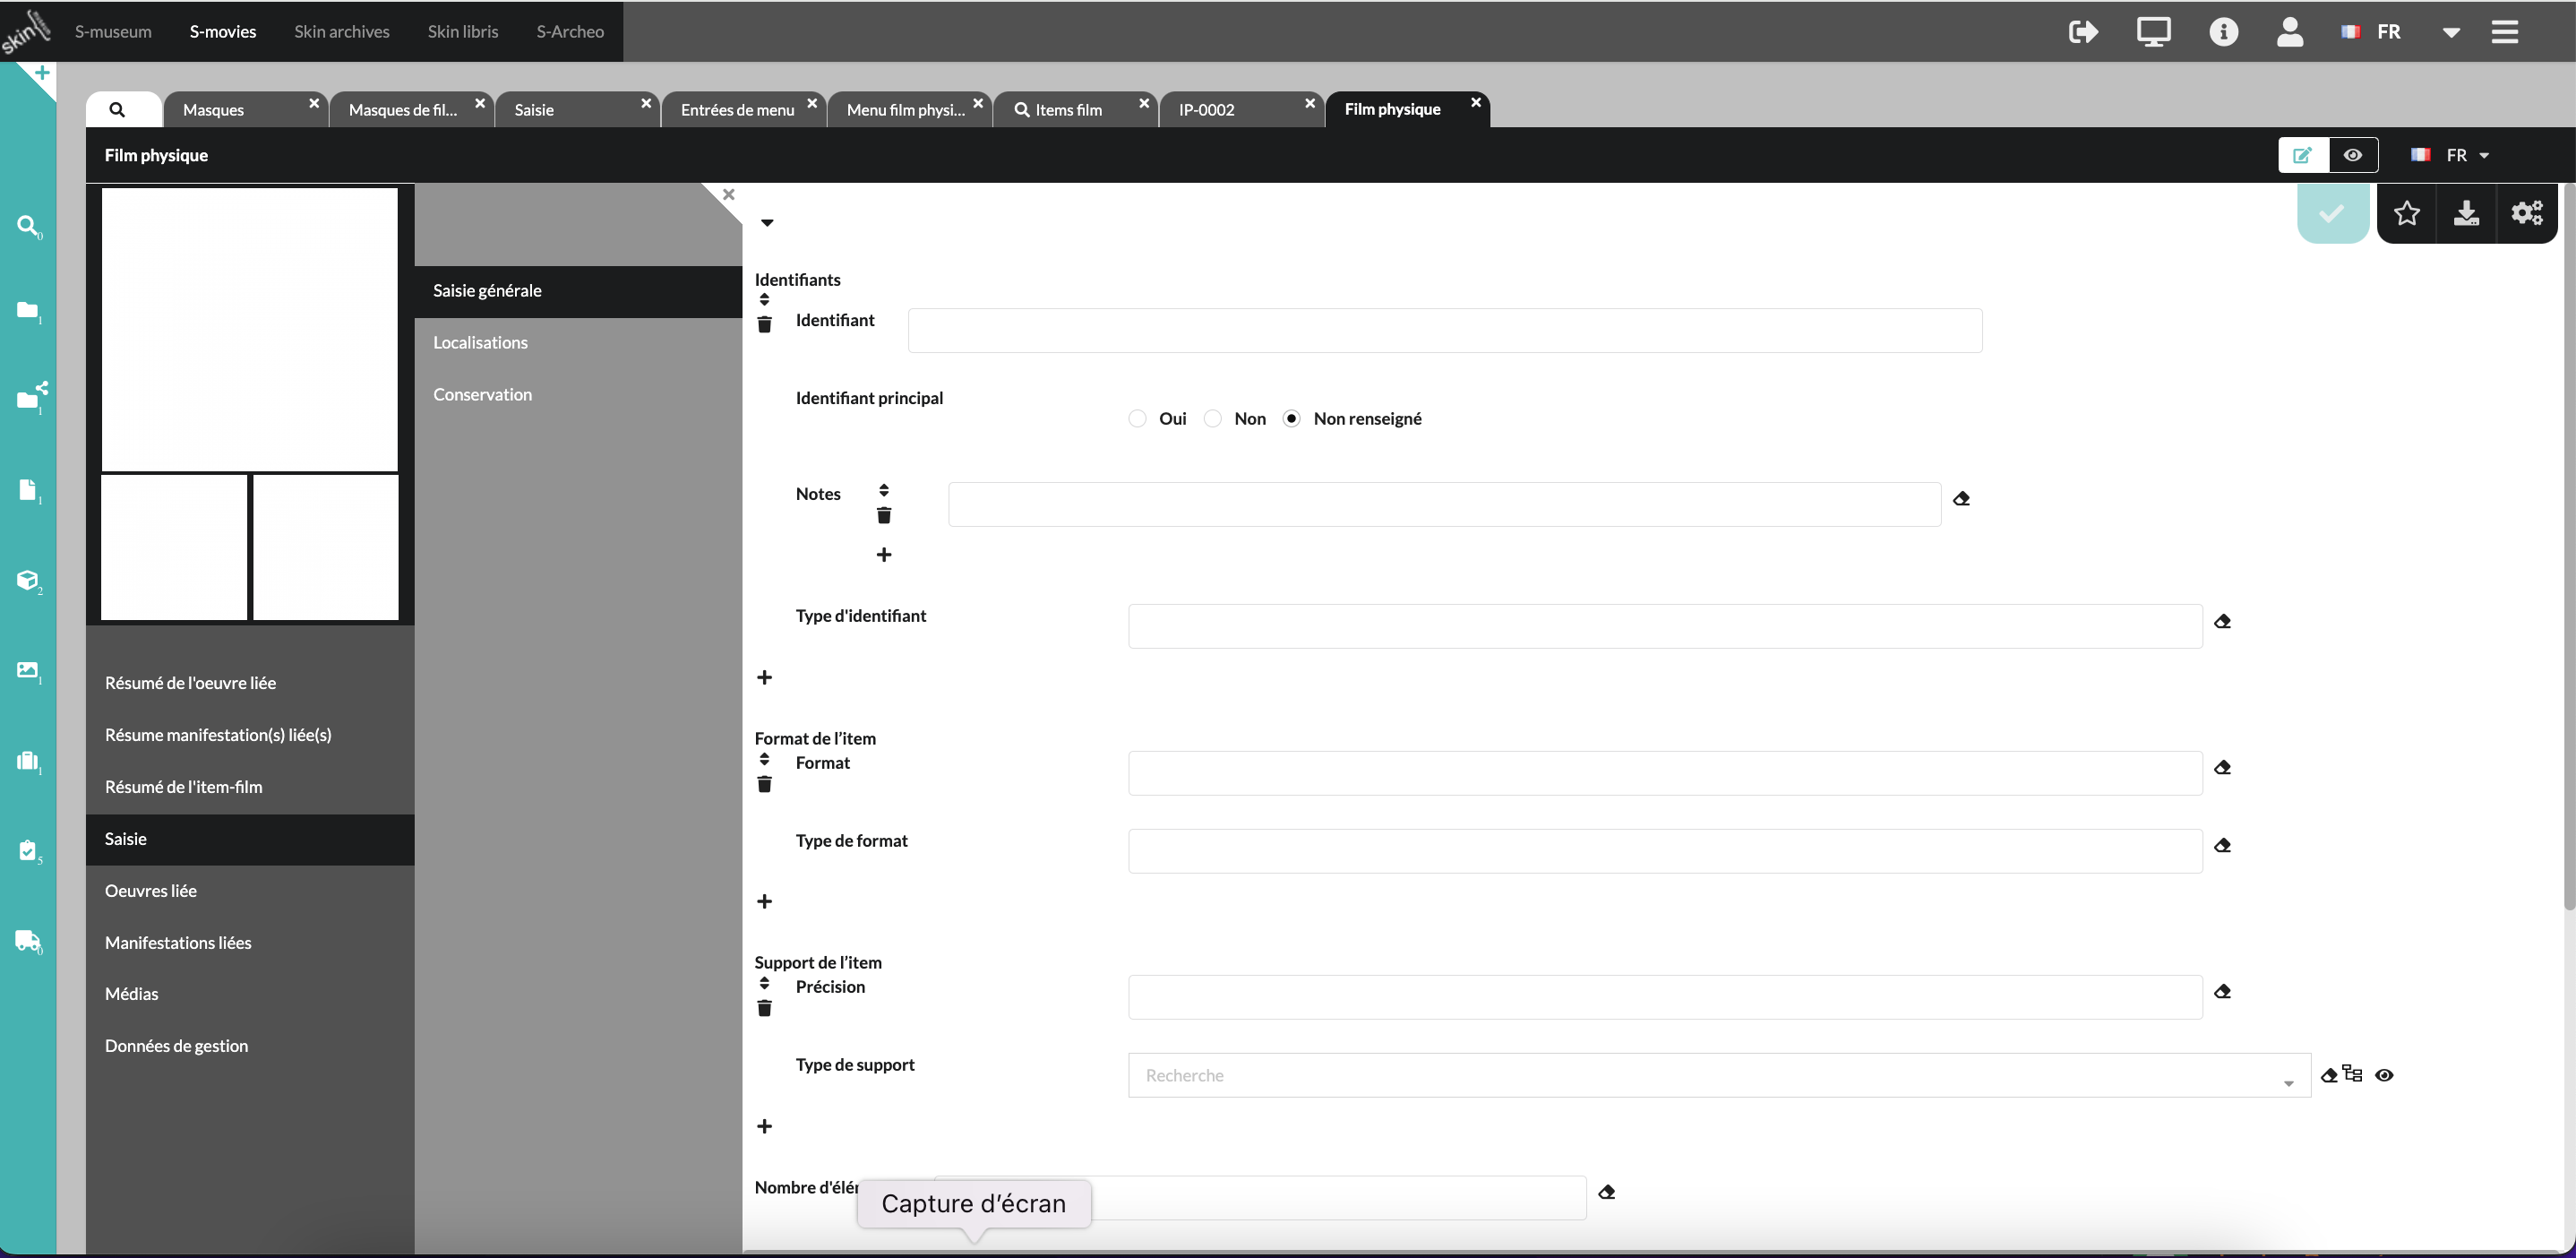
\includegraphics[width=1.0\textwidth]{images/image4.png} 
	
	\caption{Affichage du menu d'une notice de film physique à la saisie} 
	
	\label{figAffichageMenu} 
	
\end{figure}


Ce système d’organisation des masques de saisie au sein de menus permet également d’effectuer des liens avec d’autres types de notices et donc d’autres entités du FRBR. Par exemple la capture d'écran suivante \ref{figMenuGrilles}, montre que dans un menu de film physique, les onglets Œuvre liée et Manifestations liées permettent d’obtenir une grille de recherche, au sein d’une notice de film physique, affichant l’Oeuvre liée au film et les Manifestations dont il découle. 

\begin{figure}[htbp] 
	
	\centering 
	
	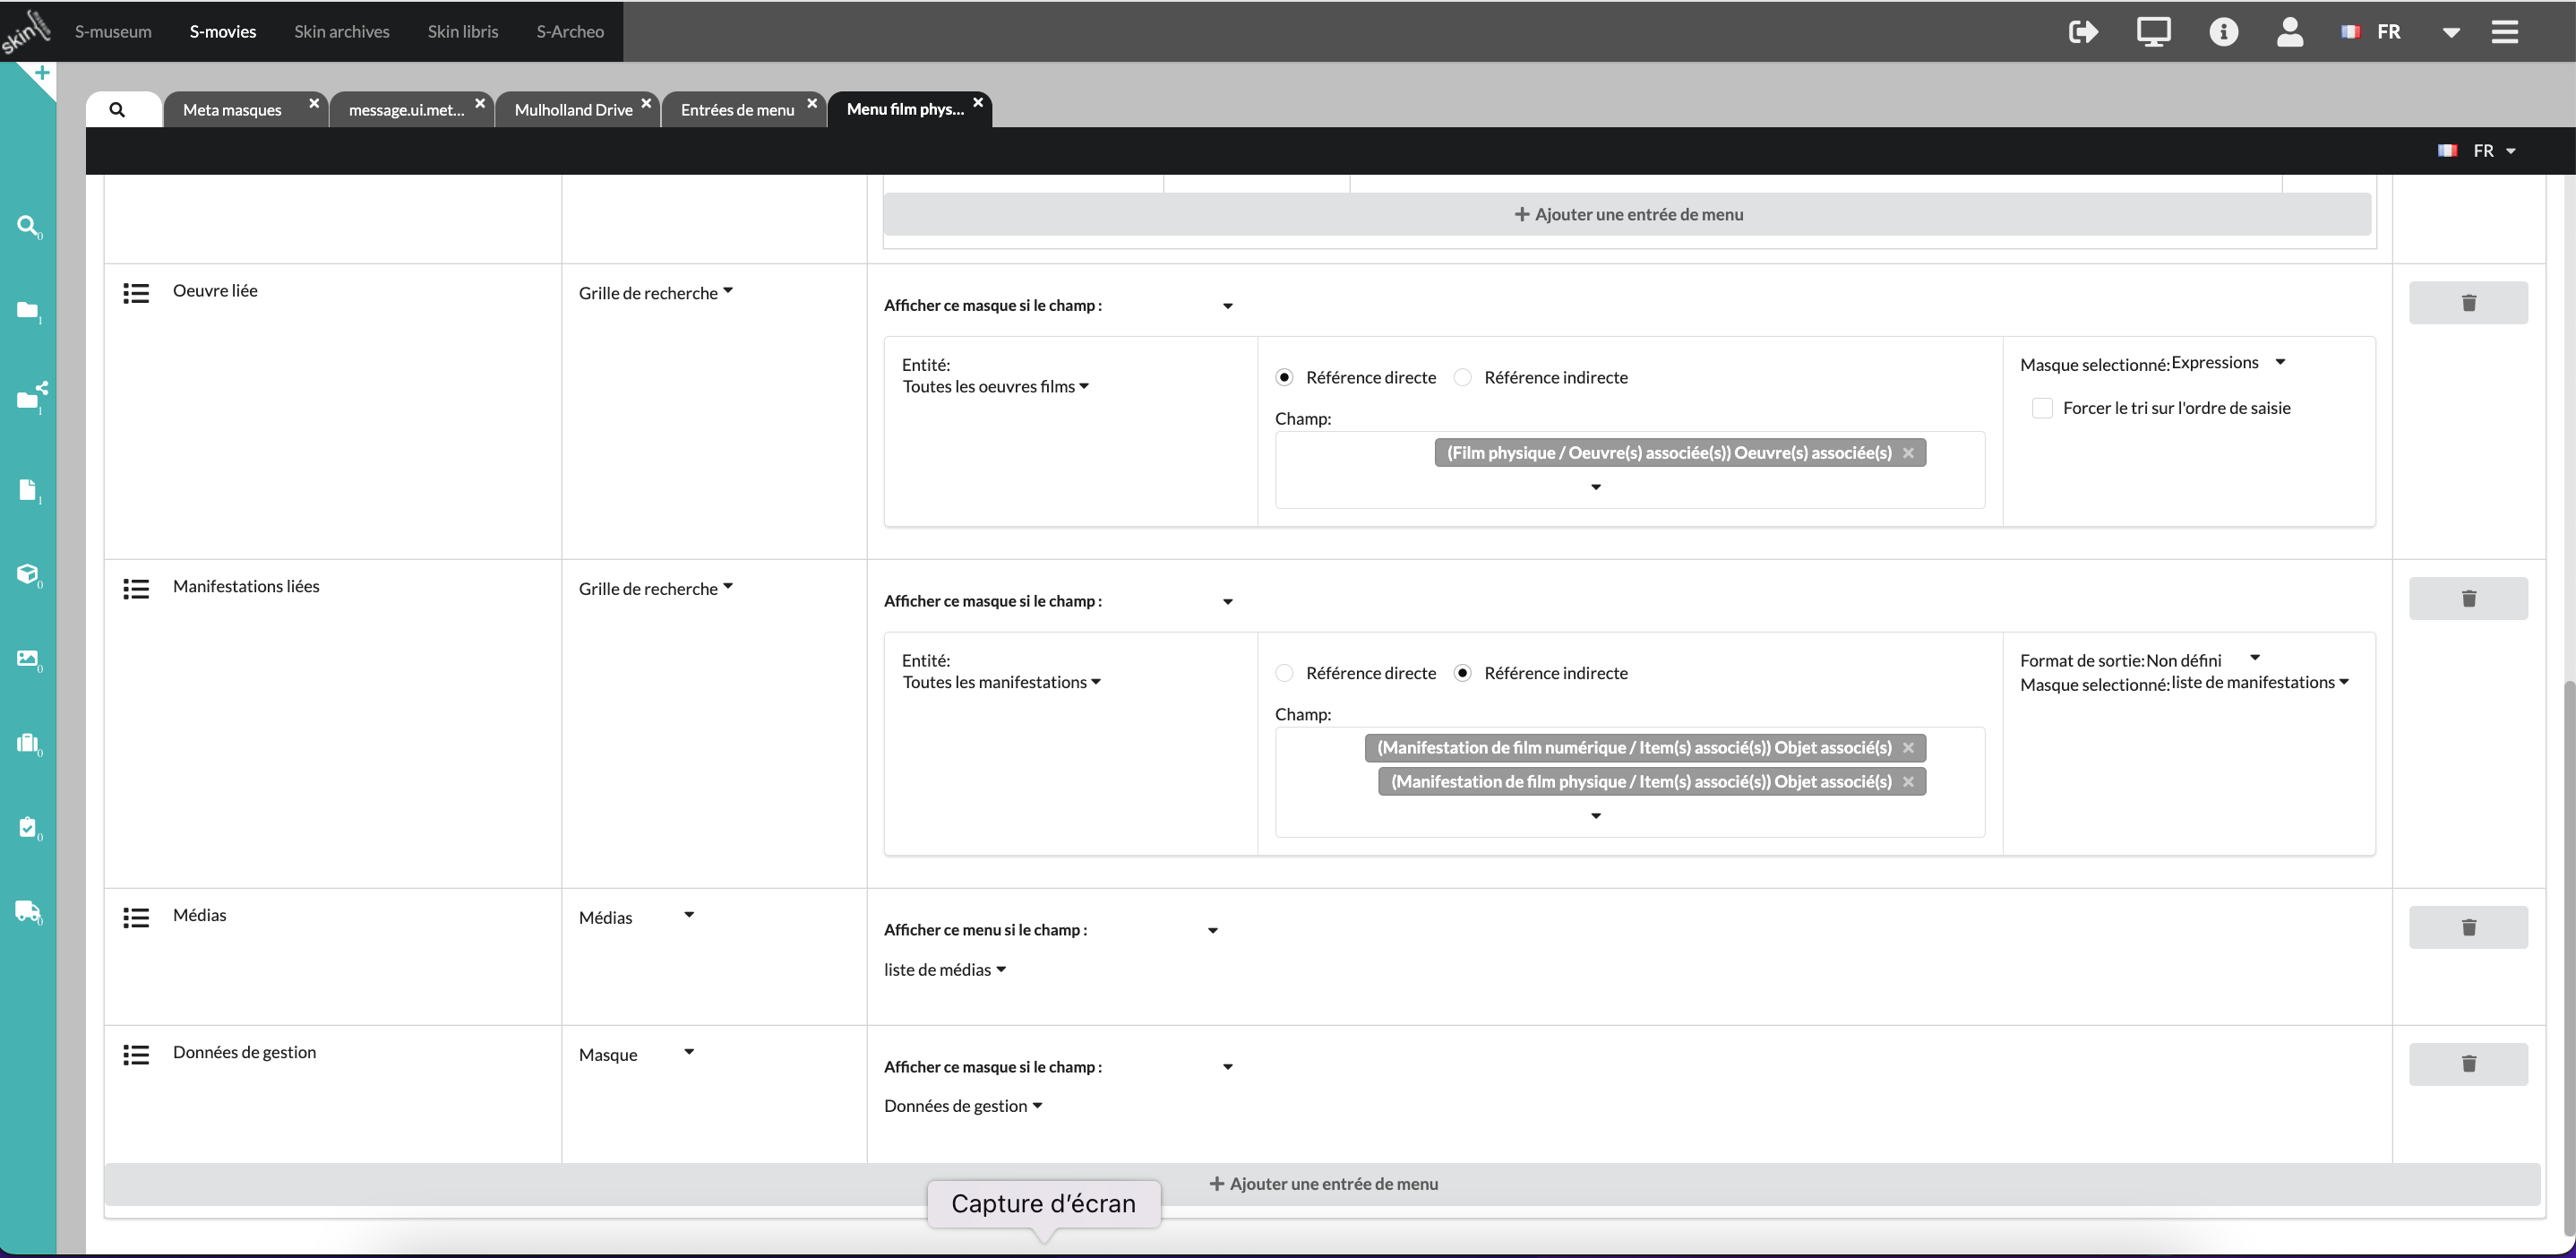
\includegraphics[width=1.0\textwidth]{images/image8.png} 
	
	\caption{Configuration de grilles de recherche pour l'affichage des éléments liés} 
	
	\label{figMenuGrilles} 
	
\end{figure}

L’affichage pour l’utilisateur au sein de la notice de film physique est le suivant, avec d’une part, l’Œuvre liée(\ref{figOeuvresLiées}, et d’autre part, les Manifestations liées \ref{figManifsLiées}: 

\begin{figure}[htbp] 
	
	\centering 
	
	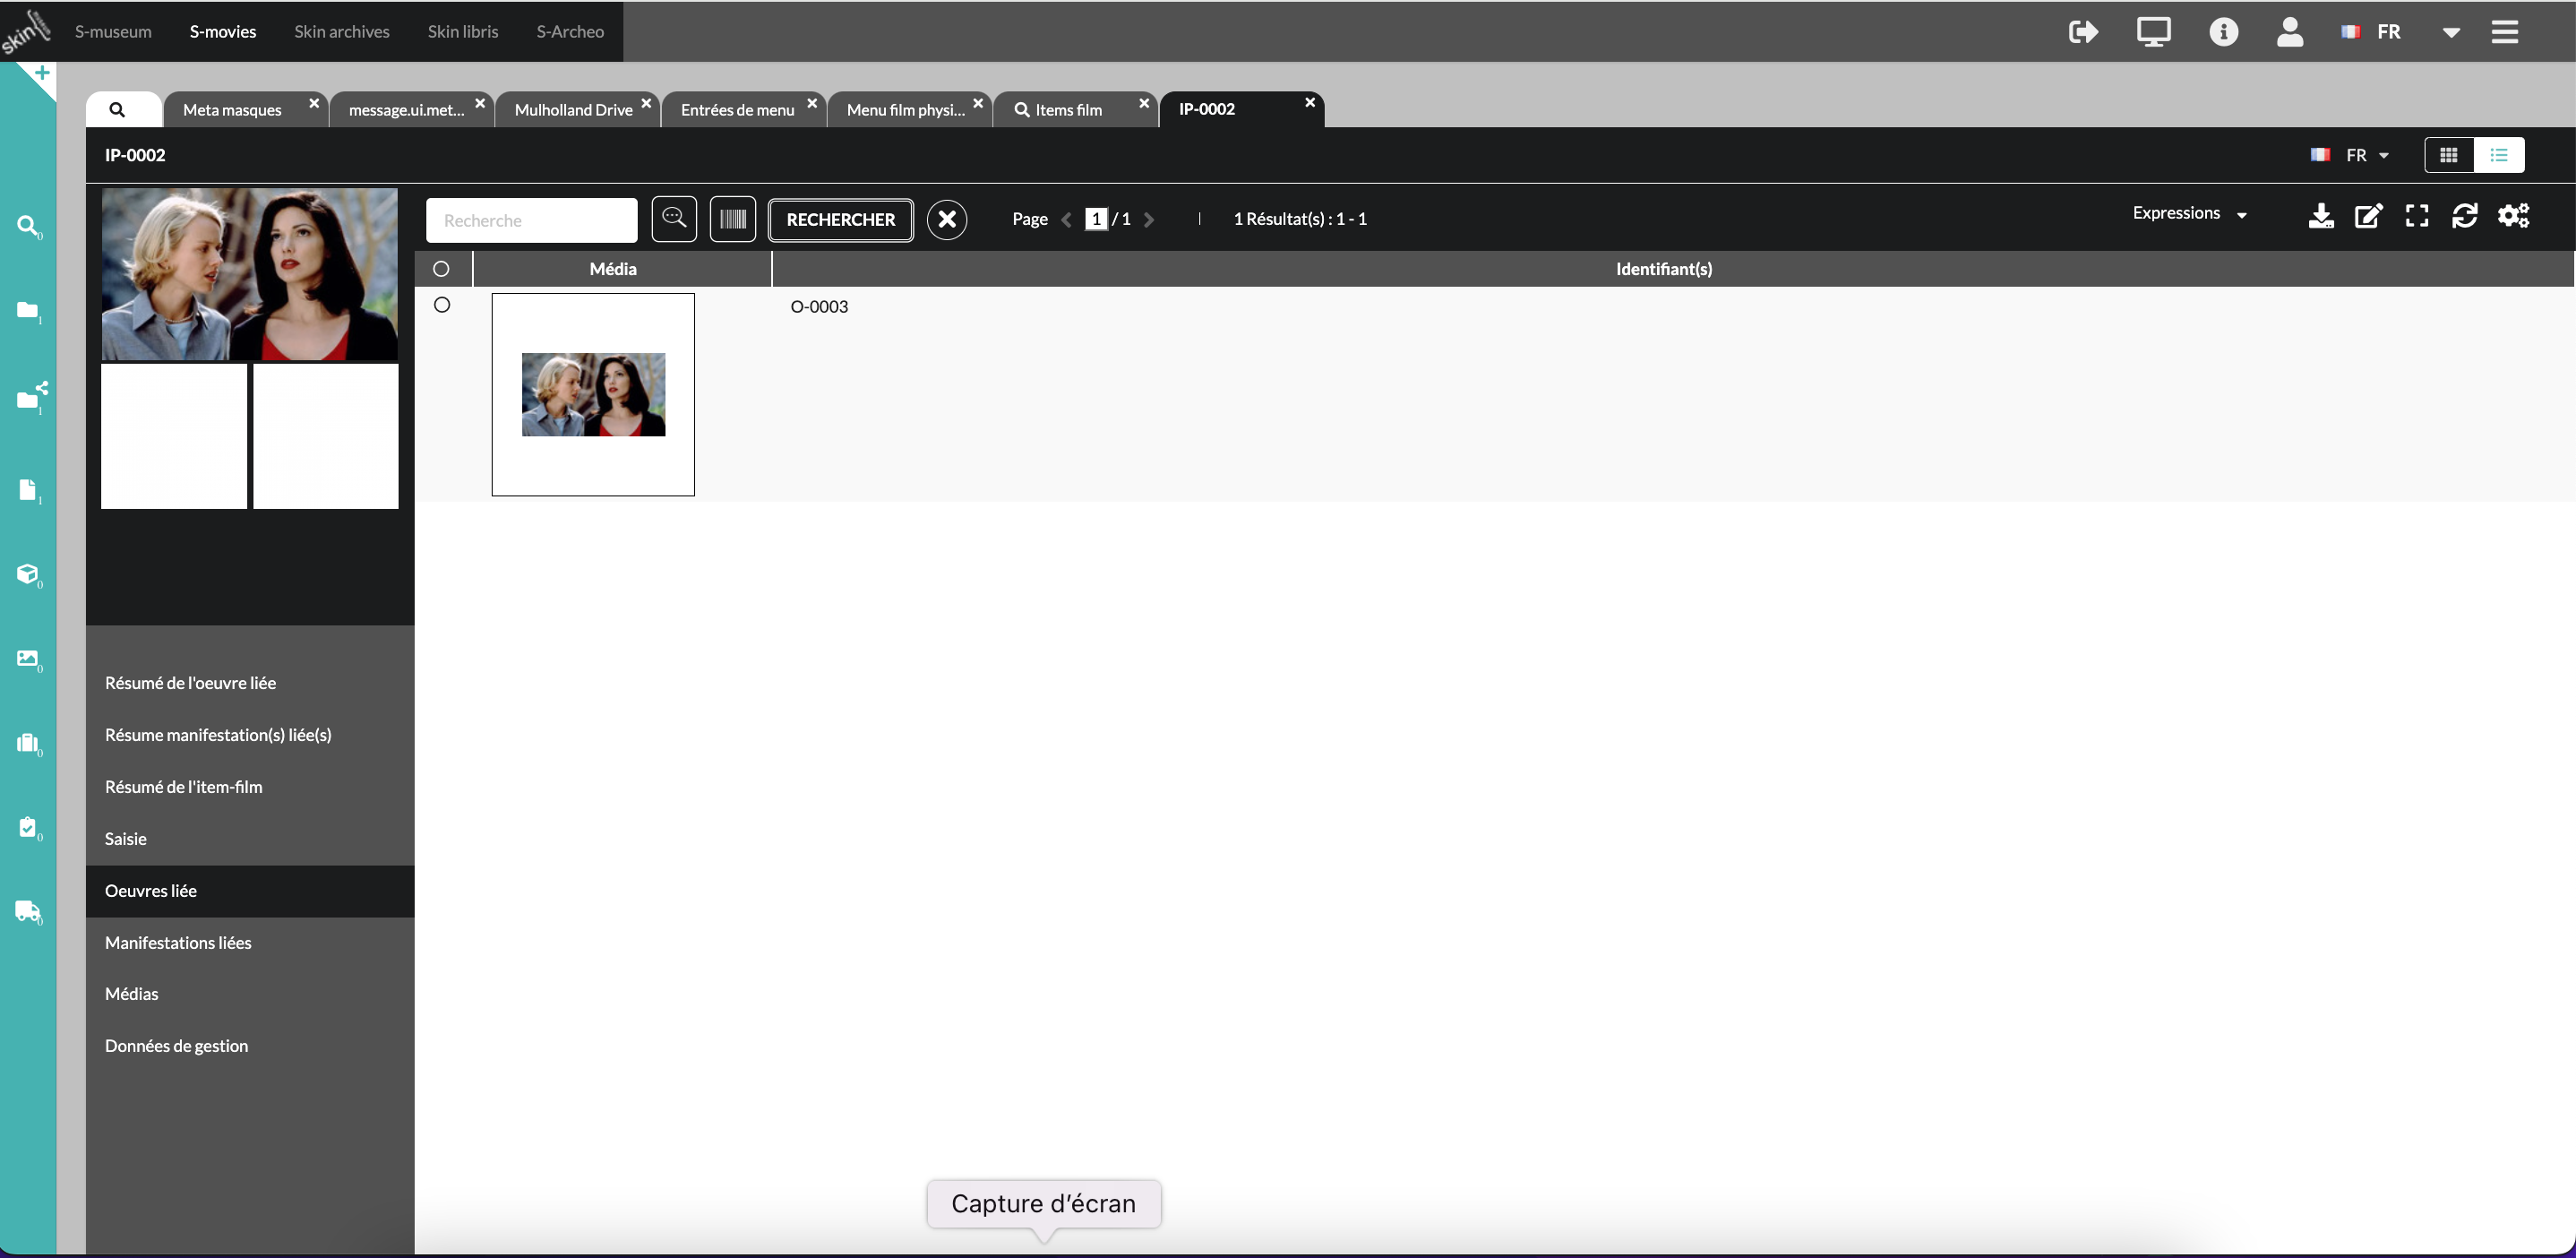
\includegraphics[width=1.0\textwidth]{images/image9.png} 
	
	\caption{Affichage des Oeuvres liées dans une notice d'item} 
	
	\label{figOeuvresLiées} 
	
\end{figure}

\begin{figure}[htbp] 
	
	\centering 
	
	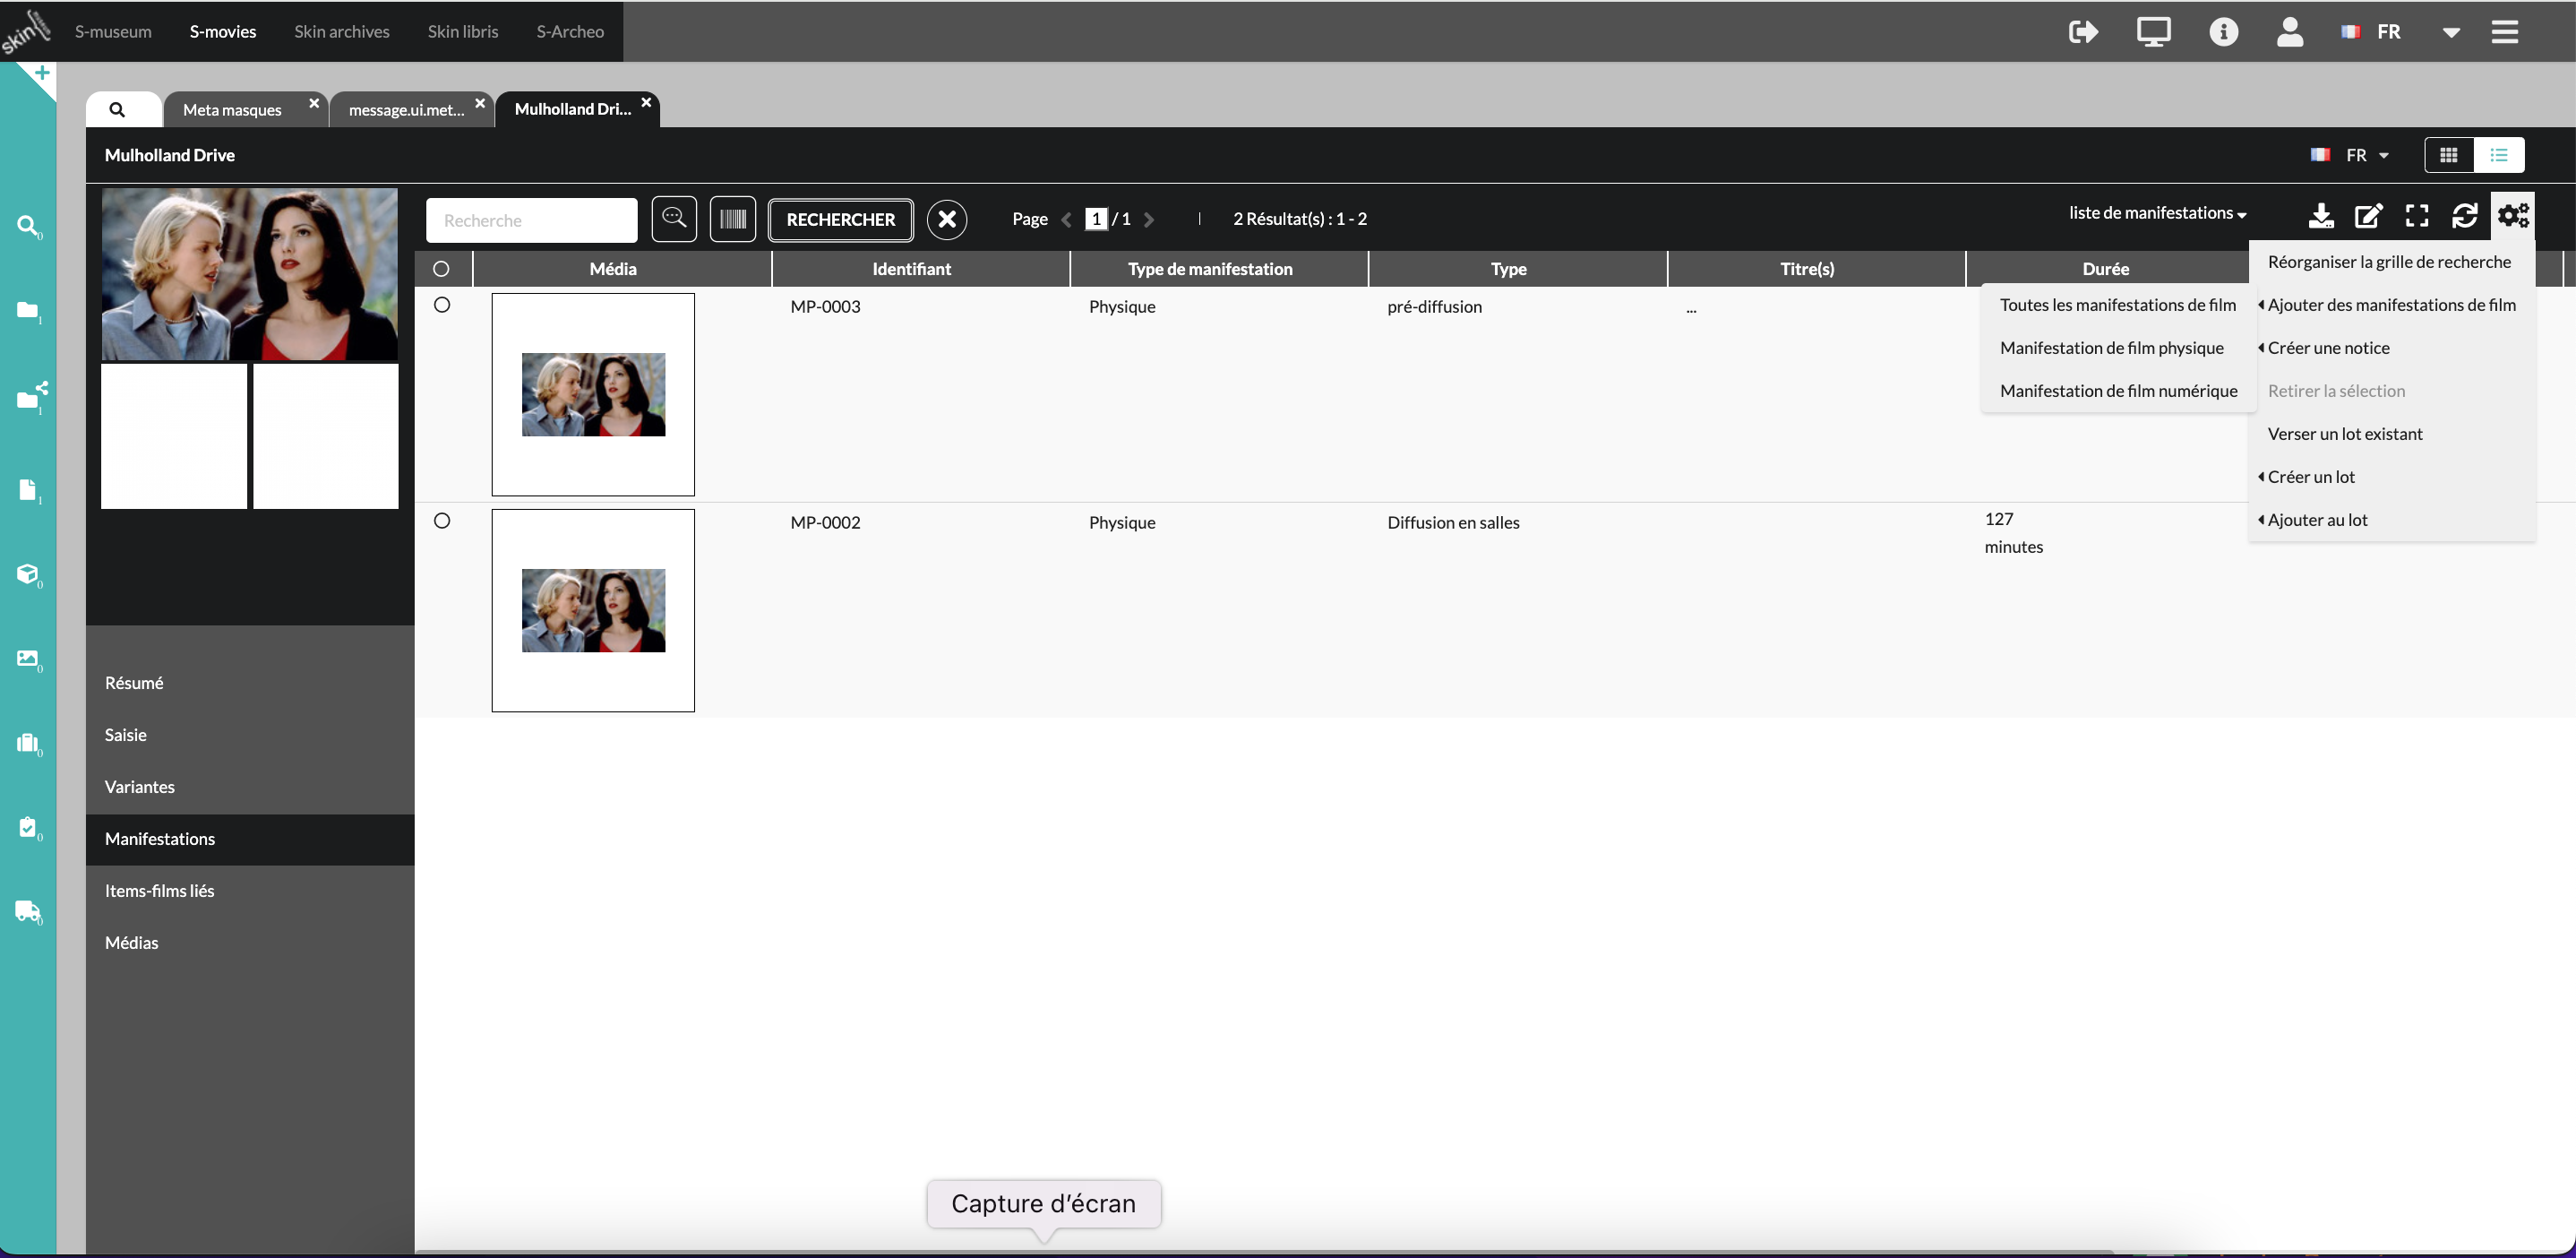
\includegraphics[width=1.0\textwidth]{images/image7.png} 
	
	\caption{Affichage des Manifestations liées dans une notice d'item} 
	
	\label{figManifsLiées} 
	
\end{figure}

Toutefois, les espaces de travail structurés sur le modèle FRBR, comme c'est le cas de S-Movies, requièrent un niveau de configuration supplémentaire, afin de concrétiser le découpage de la description en niveaux hiérarchiques. C'est le rôle des méta-masques, des formulaires de masques de saisie pouvant cibler les champs de plusieurs types de notices –et donc plusieurs niveaux du FRBR à la fois, afin d'imbriquer ces niveaux de description au sein d’une même notice. Ce système permet à l'utilisateur de saisir implicitement des éléments de description sur plusieurs niveaux du FRBR en une seule notice, permettant de surcroit au système de produire un héritage des champs d’un niveau à l’autre du FRBR.  

Concrètement, dans S-Movies, la notice d'Œuvre/Expression pointe sur les champs de l'Œuvre et de l'Expression, la notice de Manifestation pointe sur les champs de l'Œuvre, l'Expression et la Manifestation, la notice de l'Item pointe sur l'Œuvre, l'Expression, la Manifestation et l'Item. \textbf{(Faire un schéma explicatif) (citer le mode d'emploi interne ?)}. Ce mode de paramétrage de la description permet d’intégrer aux niveaux du FRBR inférieurs des champs hérités des niveaux supérieurs.  

\footnote{Notons que la présence du niveau Expression contredit le modèle FRBR préconisé par la FIAF, qui fusionne le niveau Expression dans celui d’Œuvre. Etant donné que Skinsoft possède d’autres espaces de travail modélisé sur le FRBR, comme c’est le cas de l’espace dédié à la gestion des collections bibliographiques, le niveau Expression existe seulement en théorie, mais inutilisé en pratique au sein de S-Movies.} 

Ici par exemple (\ref{figMetamasque}), un méta masque de saisie pour une notice de film physique, ciblé sur l’expression, le film physique, la manifestation de film physique, l’œuvre cinématographique : 

\begin{figure}[htbp] 
	
	\centering 
	
	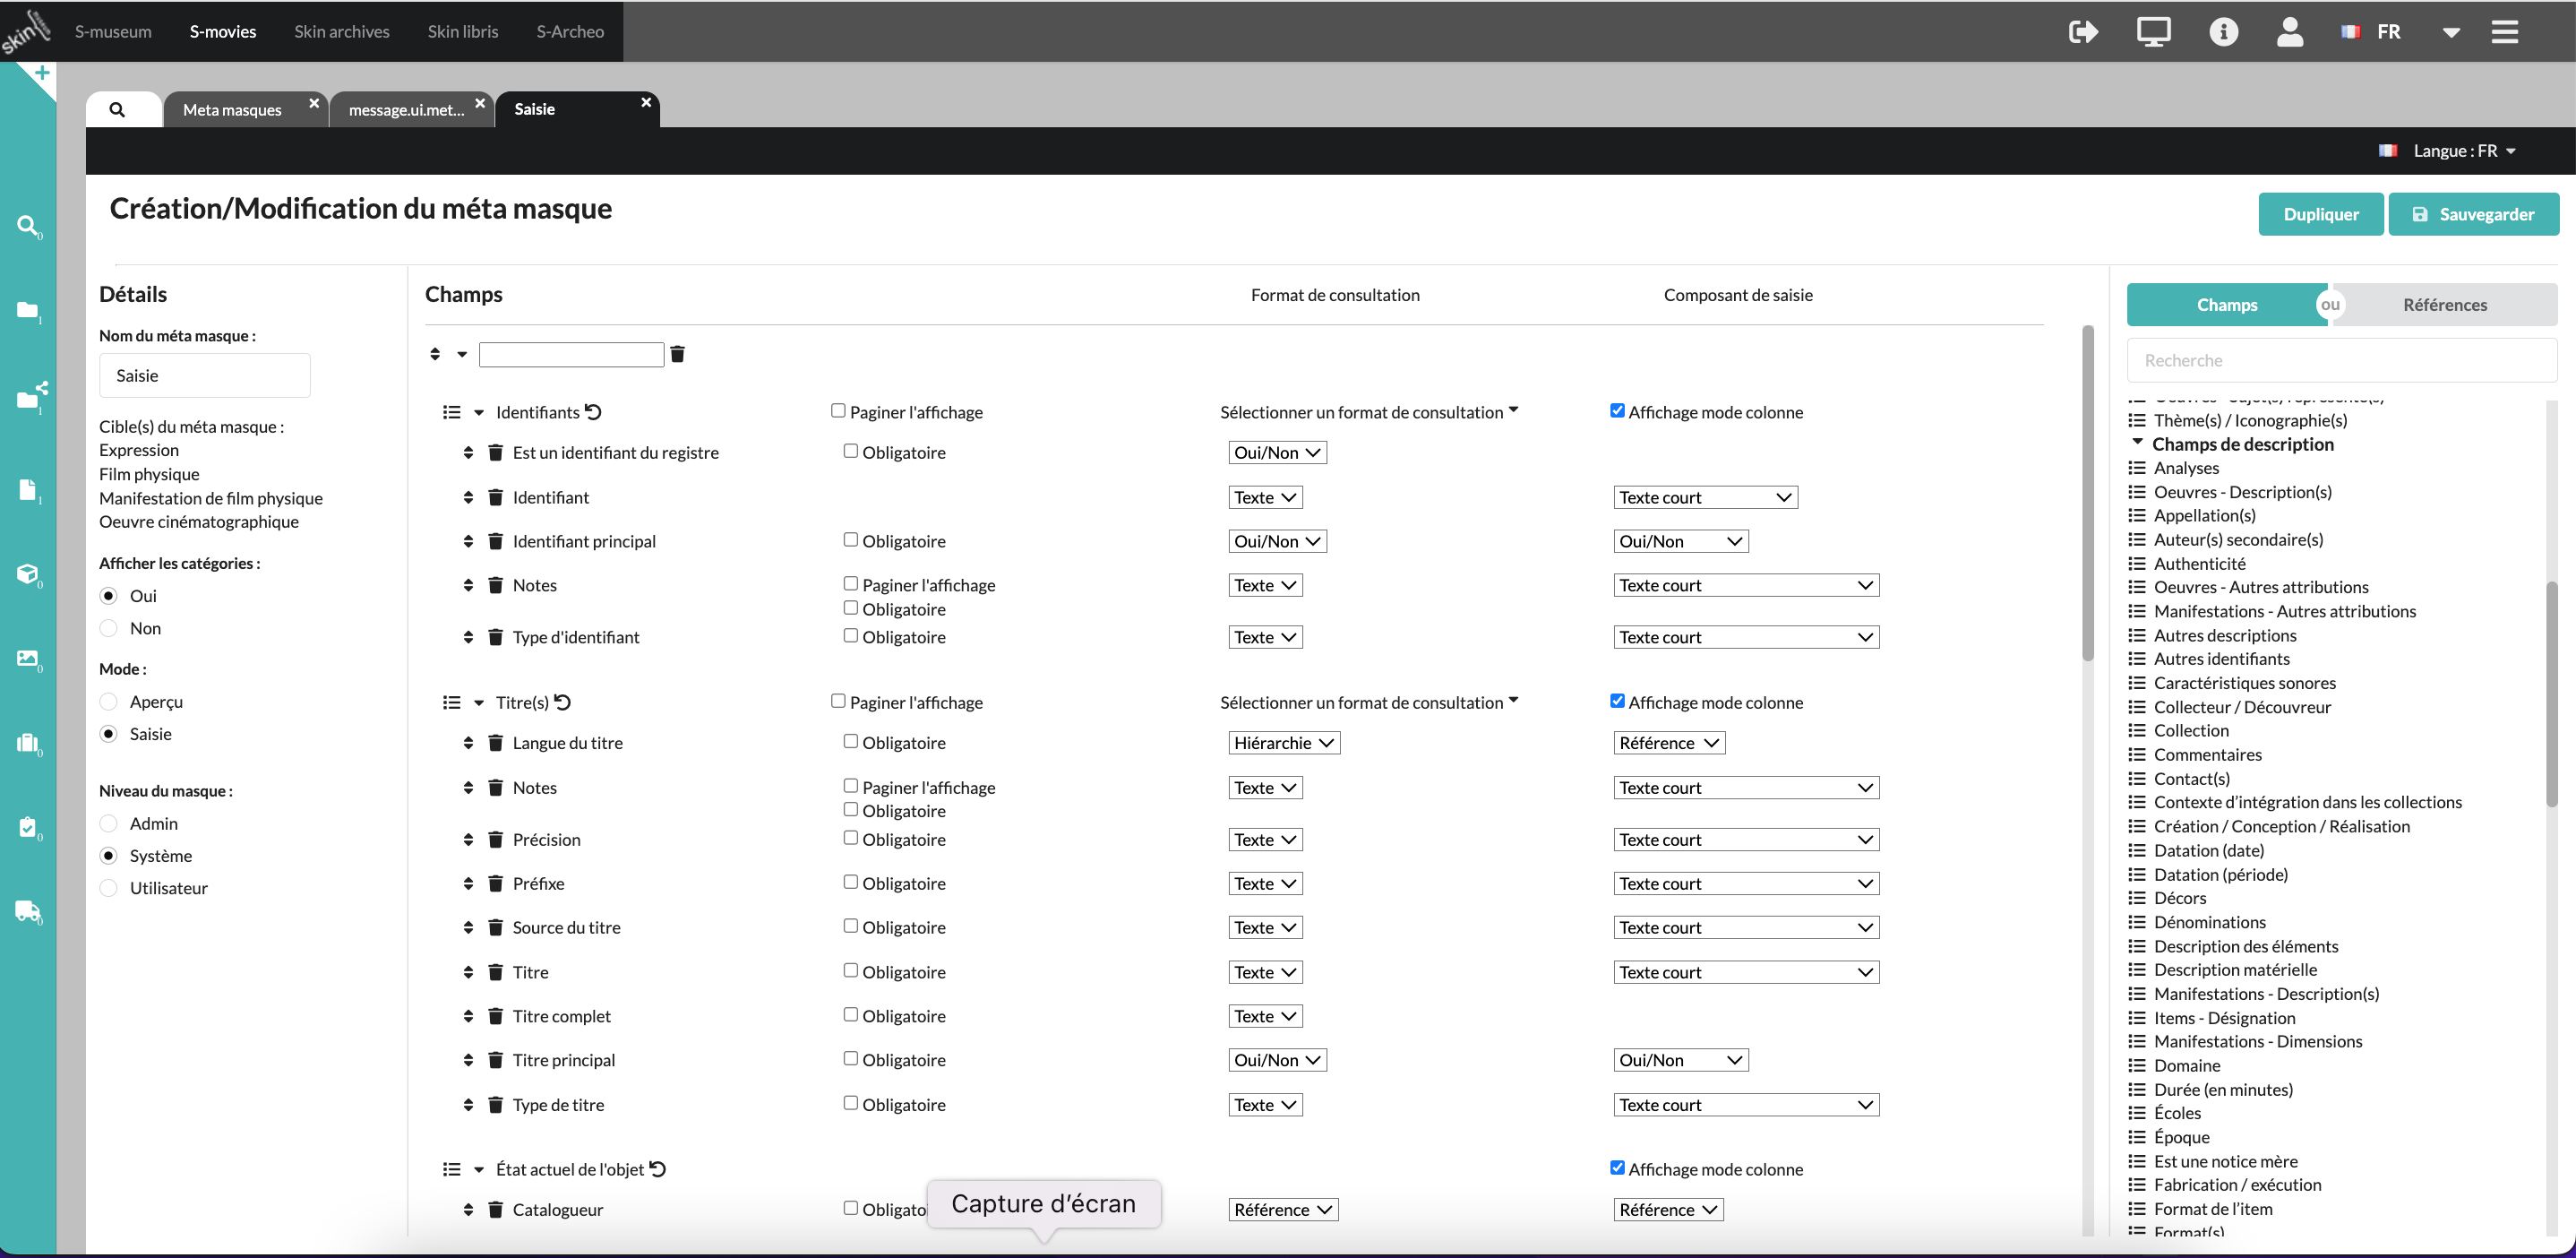
\includegraphics[width=1.0\textwidth]{images/imageb.png} 
	
	\caption{Configuration d'un méta-masque au niveau Item} 
	
	\label{figMetamasque} 
	
\end{figure}

À droite, les champs disponibles signalent à quel niveau de description ils appartiennent. Par exemple ci-dessus (\ref{figMetamasque}), le champ description appartient au niveau Œuvre, le champ dimensions appartient au niveau Manifestation.

%(: média (notice du fichier numérique, média), accessoire (modèle d'accessoire, accessoire), contenant (modèle de contenant, contenant).) 

Ces masques et méta masques créent ainsi une structure pérenne qui fait l'objet d'un paramétrage individuel qui permet d’ajuster la structure en fonction du type de collection et des usages métiers du client concerné. Ce paramétrage est défini au cours d’un travail de mapping entre les données client et la structure proposée par Skinsoft, afin de trouver un accord sur les champs qui seront utilisés pour la description des collections. L'équipe de Skinsoft organise ensuite ces champs dans des formulaires de saisie (masques et méta masques), eux-mêmes organisés pour constituer des menus de notice et des grilles de résultats de recherche. L'équipe produit également des imports de thésaurus propres aux usages de l'institution en question, afin d'assurer l'interopérabilité des données saisies. %Afin d'assurer l'interopérabilité des données, l'indexation des champs est liée à des thésaurus et des référentiels contrôlés qui ont importés au moment de la configuration de l'espace de travail pour le client. À développer  

Les fondements de l'architecture de S-Movies, doublement adaptée d’une part aux collections cinématographiques et d’autre part aux pratiques métiers spécifiques à chaque institution, constitue la condition de la qualité des données et de l’expérience utilisateur. L'enjeu de l'espace de travail est d'offrir une interface qui permette à l'utilisateur de décrire les collections en plusieurs niveaux sans difficulté et de pouvoir circuler entre ces niveaux et les liens qu’ils entretiennent. Cette circulation est notamment permise par les grilles de recherche que nous avons évoquées dont le paramétrage permet d’afficher les entités liées pour chaque notice. De plus, les différents outils de recherche permettent de circuler au sein des éléments de description indexés. (À développer ?) 

Toutefois, malgré la haute configurabilité de l’interface, l’hétérogénéité des corpus audiovisuels gérés d’une institution à l’autre complexifie le travail de mapping qui doit être effectué. En effet, la modélisation FRBR préconisée par la FIAF est un cadre qu’il s’agit d’ajuster aux pratiques spécifiques de gestion des collections, elles-mêmes adaptées au type de corpus géré. L’ajustement à des corpus audiovisuels spécifiques complexifie potentiellement la fluidité de la navigation entre les liens des différentes entités du FRBR au sein de l’interface.   

%Présentation espace S-Movies : aperçu des fonctionnalités communes et spécifiques (à placer en annexe ?): ces fonctionnalités sont chacune rattachées à un ou plusieurs niveaux du FRBR 

%- gestion des entrées : création d'un objet de collection via l'import de son média 

%- gestion des médias : associer un nouveau média à une notice de film ou un média existant 

%définir des vignettes sur les notices de films à l'aide des médias importés  

%- documents associés  

%- table collections/thématiques : regroupement des collections par thématiques : décrit le contexte de la collection, de l'assemblage des films, et présentent les items présents dans cette collection 

%- projets et mouvements : intervention, conservation, acquisitions, entrées, expositions, prêts, diffusion/programmation 

%fonctionnalités communes : gestion des contrats, évènements, interventions, expositions 

%Lien de la FIAF à S-Movies : mise en application du manuel de la FIAF, remodélisation, adaptable selon les corpus. tension public/privé 



%à bouger dans la première sous partie 

%S- Movies s'appuie sur deux normes descriptives audiovisuelles européennes : la norme EN 15744, qui définit le contenu obligatoire de description pour l'identification d'un film, ainsi que la norme EN 15907 qui découle du manuel de la FIAF et décrit une structure en couches et niveaux de données. Ces normes définissent les métadonnées essentielles pour faciliter l'échange de données et l'identification des films. \footcite{zotero-item-646} 



%Au niveau de la description des archives, il s'appuie sur la norme RDA pour la description et l'accès aux ressources. \footcite{zotero-item-646} 

%mentionner les données techniques ? : type de serveur, type de base de données 
\section{\label{I_2_B}L'inscription des corpus de données dans la remodélisation du FRBR} 

En effet, la nature du corpus audiovisuel complexifie le paramétrage puisqu'elle conditionne la capacité des données à s'adapter et s'intégrer au sein du modèle FRBR. Le modèle FRBR fait partie d'une structure fixe de l'espace de travail, avec cette séparation en trois tables de saisie (Œuvres, Manifestations, Films), dont le paramétrage peut toutefois amoindrir la rigidité. Afin d'analyser la mesure dans laquelle les corpus s'intègrent au sein du modèle FRBR, nous analyserons dans cette sous partie deux corpus de données différents gérés au sein de l’application Skinsoft. \footnote{Notons que pour des raisons de confidentialité, nous décrirons les corpus de ces institutions sans les nommer de manière explicite.}.  

Premièrement, analysons l'intégration d'un corpus de cinéma dit "classique", au sein de l'espace de travail S-Movies. Cette collection est gérée par une institution qui préserve essentiellement des films de fiction issus d'une production commerciale "grand public" depuis les débuts du cinéma jusqu'à nos jours. Cette collection est composée d’œuvres cinématographiques à proprement parlé, dont la description prend tout son sens au sein d’une modélisation selon le FRBR. La production cinématographique étant une production industrielle, les films qui en sont issus s'adaptent particulièrement bien à un modèle de données par niveaux, ces différents niveaux correspondant aux étapes de production. Ces films, après leur création, ont donc été produits et distribué à une échelle plus ou moins large. Ainsi, dans ce cas précis, le modèle FRBR est plutôt bien adapté. La réalisation du film par le montage et le tournage est décrite au niveau Œuvre, ses versions sont décrites au niveau variante, son édition et sa distribution sont décrites au niveau Manifestation, et l'exemplaire individuel du film, conservé par l'institution est décrit au niveau Item. De fait, le paramétrage décrit dans le chapitre précédent peut être réalisé sans trop de complexité au sein du cadre modélisé par le FRBR de la FIAF. (Développer + ?) 

Deuxièmement, analysons l'implémentation d'un corpus plus spécifique, celui d'une collection de \textit{rushes} documentaires muets et non montés, tournées des années 1910 à 1920. Les \textit{rushes} en termes cinématographiques correspondent à des épreuves de tournages non montées\footcite{universalis.} Ces \textit{rushes} bruts, ont été tourné dans une optique de documentation sur différents sujets, et ne sont pas destinés à une diffusion auprès du grand public. 

Dans ce cas, l'absence de montage et de distribution commerciale rend difficile l'adaptation du corpus à la modélisation prévue par la FIAF, qui structure S-Movies. Si le contexte de création du tournage peut être décrit au niveau Œuvre, les niveaux de description inférieurs sont inadaptés. En effet, en l'absence de montage, la Variante n'existe pas puisque chaque \textit{rushe} correspond à une matière brute et unique. Ainsi, l'absence de différentes versions d'une même œuvre invalide l'entité de Variante.  

De la même façon, le niveau Manifestation perd de sa pertinence descriptive puisque ces \textit{rushes} ne sont ni produits ni distribué officiellement auprès d'un public. L'inscription de l'œuvre sur un support s'effectue ici de manière unique, et en un seul et même exemplaire. Les caractéristiques matérielles pourraient donc être décrites directement au niveau de l'item.  Ainsi, d'un modèle à quatre niveaux, il ne reste, dans ce cas précis, plus que deux niveaux de descriptions exploitables : l’Œuvre et l’Item. Toutefois, notamment pour des raisons de conservation, une œuvre peut être copiée sur différents supports, physiques ou numériques. En effet, l'institution peut être amenée à produire des copies d’une œuvre sur des supports plus stables à des fins de préservation ou de diffusion en ligne, par exemple. Ces différentes matérialisations, bien qu'elles ne soient pas issues d'un processus commercial de distribution, peuvent être décrites comme des Manifestations. Telle que définie par le manuel de la FIAF, une manifestation induit en effet, "tous les médias analogiques, numériques et en ligne associés à une matérialisation particulière d'une Œuvre/Variante." \footcite{zotero-item-646}. Sa description peut alors être justifiée par des objectifs de conservation : copie, numérisation, restauration. Selon le FIAF, la description d'une Manifestation inclut les attributs suivants, -ici sélectionnés selon leur niveau de pertinence pour un tel corpus : type de manifestation, format (incluant les champs suivants : type de support, caractéristiques sonores, caractéristiques de couleur), notes.  

Or, si théoriquement le niveau Manifestation peut être décrit, en pratique dans le cas de la description de ce corpus produite par l’institution, il ne l’est pas. Est-ce que le modèle de description utilisé en pratique correspond au modèle à deux niveaux présentés brièvement par la FIAF ?  

Si au sein d'une notice d'œuvre, les champs suivants sont décrits : identification, titre, créateur, description (sujet de la prise de vue), mots clés, films associés, manifestations associées, matériel non-film associé, archives associées, bibliographie, médias, données de gestion ; la table Manifestations, en revanche, contient un nombre conséquent de notices vides. En effet, l'application Skinsoft crée automatiquement une notice de manifestation liée lorsque l'utilisateur crée une notice d'item. Dans ce cas, l’entité Manifestation devient une condition structurelle afin de maintenir la cohérence du modèle, mais perd son sens au sein d’un contexte d'indexation concret. La table des items, quant à elle, est répartie en trois catégories d'objets : bobines, cassettes ---qui constituent les films physiques--- et films numériques. Lorsqu'un même film physique est présent en plusieurs exemplaires dans la collection, les notices sont distinguées par la mention "bobine originale" et "reproduction". Les notices de films physiques contiennent une description matérielle sur le support et la condition de ce support. Elles mentionnent également les collections liées vers d'autres Items et Œuvres, vers des médias et des documents. La manifestation référente est tout de même mentionnée mais il s'agit, nous l'avons évoqué, d'une notice factice. Enfin, les films numériques décrivent le support original depuis lequel la numérisation a été effectuée, les raisons de la numérisation ---par exemple, copie de sauvegarde---, et l'item physique qui a fait l'objet de cette numérisation.  

Par ailleurs, un élément précis a retenu notre attention dans le cadre de notre étude. En effet, la présence de \textit{time-codes} ---marqueurs temporels dans des notices de films numériques, traduisant l'inscription de la copie numérisée dans une œuvre plus large. En effet, certaines Œuvres-rushes, dont les modalités matérielles sont décrites dans une notice de film physique, ont été divisées en extraits puis numérisées. Étant donné que les Œuvres conservées sont des rushes non montés, cette division en extraits a pour but de réaliser une forme de montage et de rendre ces films intelligibles via une diffusion en ligne. Ainsi, la plupart des films numériques gérés au sein de S-Movies sont issus de ce découpage depuis les rushes originaux. Les repères temporels expriment le rattachement précis de l'item numérique au sein d'un item physique.  

Ainsi, la modélisation de données adaptées à ce corpus audiovisuel précis s'apparente à un modèle hiérarchique à deux niveaux, celui d'une Œuvre matérialisée dans une Manifestation/Item, fusionnés en une seule entité. Cette hiérarchie à deux niveaux est brièvement décrite dans le catalogue de la FIAF en tant qu'exemple, mais ses modalités ne sont pas détaillées. (À développer?) 

\begin{figure}[htbp] 
	
	\centering 
	
	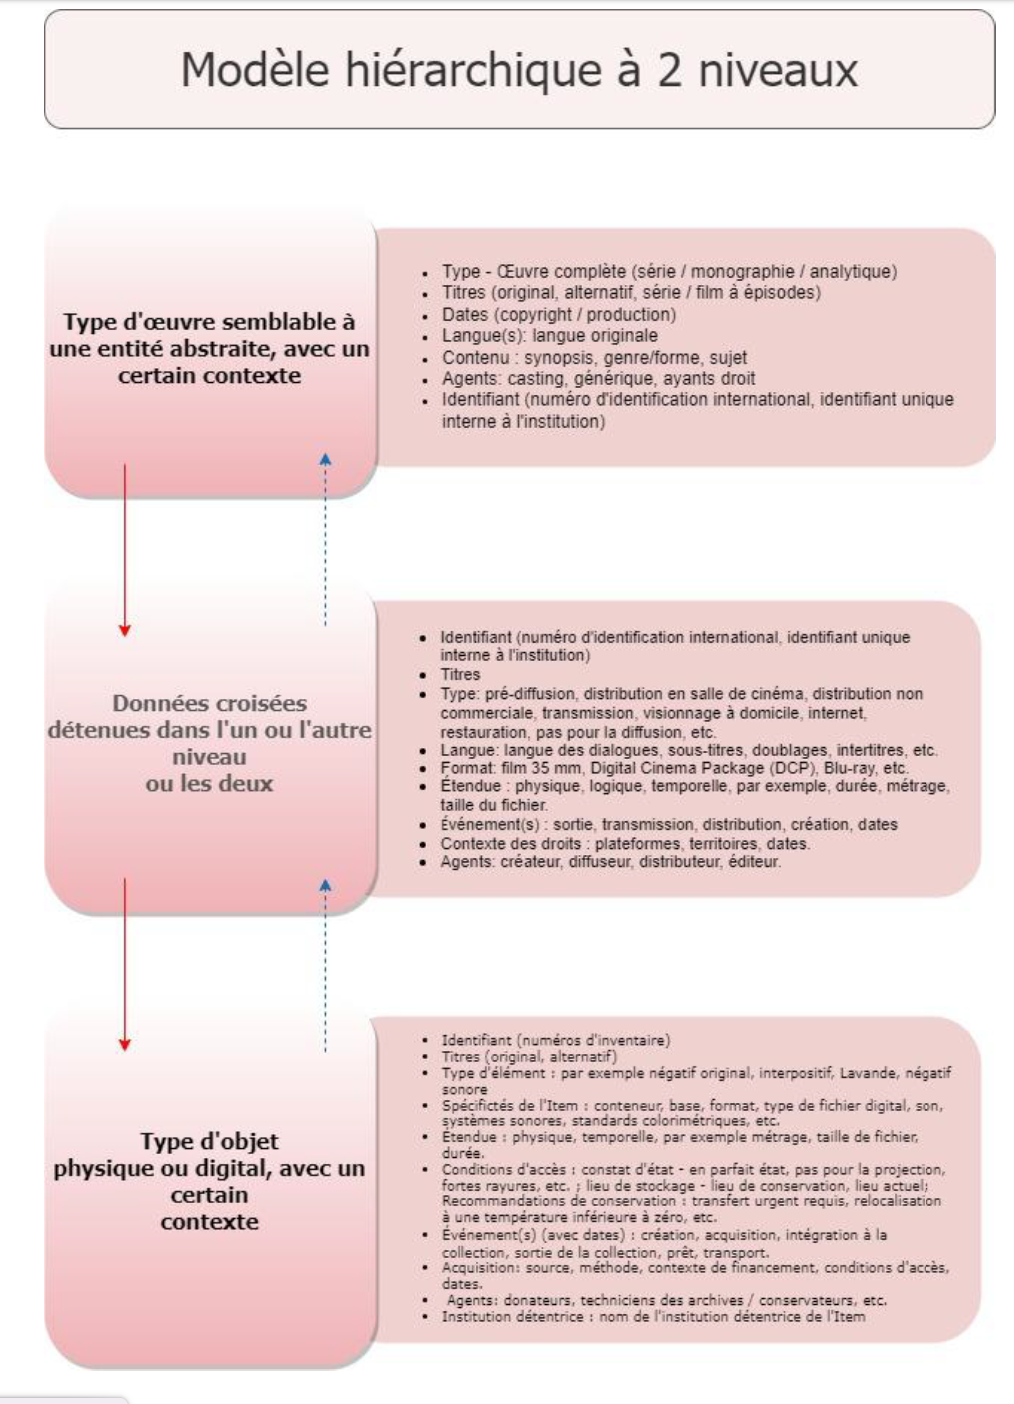
\includegraphics[width=1.0\textwidth]{images/imagec.png} 
	
	\caption{Modèle hiérarchique à deux niveaux schématisé par le manuel de la FIAF} 
	
	\label{figModele2Niveaux} 
	
\end{figure}

Développer davantage le schéma de données que ça produit dans l’appli client ? Avec un schéma ? À partir des captures d’écran suivantes : schématiser les liens complexes entre éléments pour le corpus en question  

Par exemple : Une notice Œuvre est liée à un item numérique, lui- même lié à un ou plusieurs films physiques : cassette, bobine, avec le time code mentionné pour traduire la place de l’extrait/film numérique au sein de ces supports physiques.  

Les films physiques : contiennent la liste des films numériques qu’ils ont pour extrait + les différentes reproductions du film physiques sur d’autres supports physiques : plusieurs bobines, plusieurs cassettes (à des fins de conservation)  

Si l'espace de travail S-Movies parvient à maintenir le modèle du FRBR en trois niveaux principaux pour les corpus audiovisuels standards, la description de corpus plus spécifiques éclipse notamment le niveau Manifestation pour ne conserver qu'une hiérarchie à deux niveaux. L’analyse de l’inscription d’un corpus donné au sein de la modélisation de données proposée par S-Movies soulève des interrogations sur la fluidité de la navigation de l’utilisateur au sein de l’interface.  En effet, le caractère brut du corpus observé nécessite une description fine du contenu afin de restituer une intelligibilité, d’habitude produite par le montage, qui doit être prévue par une saisie ergonomique au sein de l’interface. Afin d’adapter l’espace de travail à des corpus aussi spécifiques, l’éditeur Skinsoft engage notamment une démarche de refonte de S-Movies, dont l’objectif est de repenser d’une part l’interface fondée sur le FRBR, et d’autre part d’intégrer des fonctionnalités innovantes d’indexation automatique afin d’assister l’utilisateur dans la description des collections. C’est dans ce contexte d’innovation technique que s’inscrit notre stage, au cours duquel nous avons étudié l’usage de S-Movies afin d'en améliorer l’expérience utilisateur, et ainsi préparer l’implémentation de fonctionnalités automatiques pour la description des collections audiovisuelles. 
\section{\label{I_2_C}Vers une refonte de S-Movies} 

Si le cadre posé par la modélisation FRBR s’avère limité pour des collections spécifiques telles que celles que nous avons analysé, le modèle induit des difficultés plus globales au niveau de l’interface et de la navigation utilisateur. Le FRBR est fondé sur des besoins utilisateurs dont l’objectif serait “d’identifier, sélectionner et acquérir” efficacement l’ensemble des éléments décrits et répartis entre différents nie=veaux hiérarchiues \footcite{zotero-item-646}. Ces besoins semblent respectés au sein de l’interface S-Movies, via la navigation permise entre les entités et les outils de recherche disponibles. Toutefois, une double complexité subsiste dans l’implémentation de la modélisation FRBR au sein d’une interface. D’une part, il reste complexe de mettre en place une interface intuitive permettant à l’utilisateur de connaître immédiatement le rôle descriptif de telle entité du FRBR et sa place au sein de la hiérarchie du modèle. D’autre part, la visualisation des liens entre les entités du FRBR reste limitée, puisqu’elle supposerait des développements supplémentaires innovants tels que la visualisation en graphe, par exemple.  

Parmi les complexités d’interface révélés par l'expérience utilisateur, certains éléments semblent anodins. Par exemple, l’affichage d’une hiérarchie inversée du FRBR dans le menu de l’application, pouvant nuire à l’intuitivité du rôle de chaque entité pour la description des collections. En effet, au sein du menu, les tables sont présentées de telle manière à ce que le plus bas niveau du FRBR (l'item) apparaisse en haut, suivi de la manifestation et du plus haut niveau (l'œuvre). Cet affichage visuel descendant peut induire en erreur l'utilisateur sur la navigation hiérarchique à employer au sein du modèle. De plus, au sein de S-Movies le plus bas niveau de la hiérarchie (l’Item) est désigné par la notion de “Film”. Or, dans un contexte cinématographique, le film peut communément désigner à la fois une œuvre et un item individuel. La notion de film n'évoque pas le caractère unique et individuel de l'exemplaire tel qu'il est défini par le manuel de la FIAF. Une autre confusion terminologique potentielle peut être créée par la présence de la notion d'Expression, alors même que ce niveau, issu du modèle FRBR bibliographique, est fusionné dans celui d'œuvre.  

La visualisation des liens entre les entités descriptives au sein de l’interface est également motrice d’améliorations au sein de l’espace de travail. L'interface actuelle permet, après configuration, de visualiser les liens d’une notice avec d’autres notices issues de niveaux différents du FRBR. Or, il serait pertinent pour l’utilisateur d’avoir la possibilité de visualiser les liens entre entités à un niveau plus large, et de manière graphique. Par exemple, il serait pertinent de pouvoir visualiser, au niveau d’une notice Œuvre, l'ensemble des manifestations dans lesquelles elle est matérialisée, ainsi que tous les exemplaires issus de ses manifestations respectives et conservés par l’institution. Cette visualisation des liens pourrait être étendue de manière plus large au niveau de la table d’une entité, ou de celui de la collection de l’institution.  

Par ailleurs, la mise en place de liens indissociables entre entités prévus par le modèle FRBR nécessitent, au sein de l’interface, des configurations spécifiques complexes. En effet, l’indissociabilité des liens entre les entités suppose que l’interface rende obligatoire pour l’utilisateur l’association de certaines notices entre elles. Par exemple, un Item doit obligatoirement être lié à une Manifestation et/ou à une Œuvre. Or l’obligation de ces liens n’est pas encore prévue par l’interface, laissant ainsi la possibilité à l’utilisateur de créer un Item sans Œuvre liée par exemple. De même, l’interface permet par exemple la suppression d'une notice Œuvre et de tous ses éléments liés (notices de Manifestations et d’Items), sans avertissement préalable. 

Ces difficultés d’interface sont en réalité issues de la complexité de traduire un cadre de modélisation défini, en termes d’expérience utilisateur. Cette traduction est cruciale afin d’assurer la qualité des données indexées au sein de l’interface. En effet, l’intuitivité de l'interface permet à l'utilisateur de diviser la description d’un objet entre les différents niveaux prévus par l’application, et d’associer ces niveaux entre eux afin qu’ils soient requêtables au sein de l’interface. L’absence d’intuitivité peut notamment empêcher l’héritage des données entre les différents niveaux, dans le cas d’une notice dépourvue de liens, par exemple. L’interface doit ainsi assurer la qualité des données en instaurant une circulation intuitive au sein du modèle FRBR.  




 



Transition interface utilisateur > et projet IA : 

L’analyse de l’espace de travail S-Movies a permis d’étudier la manière dont le modèle FRBR structure l’architecture des relations entre entités, permettant la description des collections. Toutefois, la qualité de ce système repose moins sur la description que sur l’indexation des collections. L’indexation désigne la mise en place d’une description contrôlée et normalisée en lien avec des thésaurus, par exemple, permettant de concrétiser les besoins utilisateurs fondateurs du modèle FRBR. En effet, c’est l’indexation qui permet à l’utilisateur d’accéder à des objets de collection via des requêtes contenant des éléments de description indexés. Cette opération d’indexation peut s’avérer complexe et chronophage dans le cas de corpus tels que nous avons analysés, poussant un éditeur d’outil de gestion des collections à proposer des outils d’assistance automatique. En effet, Skinsoft souhaite par exemple intégrer à S-Movies des fonctionnalités d’indexation fondées sur l’intelligence artificielle capables d’effectuer une segmentation d’extraits vidéo et de décrire ces extraits afin de les indexer au sein du modèle FRBR.  

%Or, pour pouvoir mettre en place un modèle d'intelligence artificielle qui automatiserait des pratiques métier d'indexation, il est nécessaire de clarifier en amont la définition de la hiérarchie des niveaux FRBR au sein de l'application, et des liens qu'ils entretiennent. En effet, l'interface graphique constitue bien une définition et une traduction du modèle FRBR pour les utilisateurs. Si un modèle d'IA est mis en place alors que des incohérences subsistent, l'automatisation de l'indexation qui, de fait, accélère son processus, produira des erreurs de données à plus large échelle. 















. 